\chapter{二维材料异质结生长机理的研究}
\section{引言}
石墨烯作为经典的二维材料,由于独特的晶体结构和电子结构特性,在超导,量子计算、量子晶体管等方面具有独特的优势\citing{RN1068-2020,RN1071-2021,RN1065-2013,RN997-2007,RN1008-2015}。而要将石墨烯真正运用到电子器件之中,并且与现行的平面硅工艺兼容,研究者需要将石墨烯转移到\cemb{SiO2}等绝缘衬底的表面。而石墨烯在\cemb{SiO2}为代表的绝缘衬底表面通常以无序的状态存在,破碎的晶格使得石墨烯在这些绝缘衬底的表面难以完全发挥出理论上限。
而作为二维材料中的绝缘体,六方氮化硼\cemb{h-BN}在具有较大的带隙的同时也保有二维材料高质量面内结构的特点。趋近完美的二维晶体结构使得\cemb{h-BN}在禁带内具有极低的缺陷态密度以及较高的击穿电压。同时,\cemb{h-BN}与石墨烯之间的晶格失配只有\SI{2}{\percent},这使得\cemb{h-BN}非常适合搞高性能电子器件中替代\cemb{SiO2}作为石墨烯的衬底材料 \citing{RN959-2010}。这种将不同的二维材料纵向堆叠起来可以制成纵向异质结,层与层之间由较弱的范德华力或准范德华力连接。以二维材料所组成的异质结能够结合不同二维材料优异的物理特性,使得二维材料在多种新型器件中能够最大化的发挥其独特的优势。许多新奇的物理现象已经在石墨烯和\cemb{h-BN}的纵向堆叠而成的二维异质结被研究者所发现,如在外磁场下电子和磁场场强的霍夫斯塔特蝴蝶分型图像\citing{RN1286-2013, RN1287-2013, RN1285-2013}。同时,石墨烯/\cemb{h-BN}纵向二维异质结具有非常好的制备质量,石墨烯高度可调的物理特性,以及二者之间存在的周期性的摩尔超晶格。这些都使得石墨烯/\cemb{h-BN}纵向二维异质结成为了一个非常好的观测新奇量子现象的基础平台。

然而,虽然机械剥离的方式能够制备具有极高质量的石墨烯/\cemb{h-BN}纵向二维异质结,但受限于较低生产效率和高昂的合成成本,剥离的方式很难应用于大规模的二维材料的生产制备。而常用于大规模低成本制备石墨烯的化学气相沉积法通常需要\cemb{Cu}等金属衬底的催化作用的协助。由于\cemb{h-BN}对于甲烷等含碳前驱体裂解反应的催化活性远不及金属衬底,石墨烯在\cemb{h-BN}上直接生长的速率同样也远低于在金属衬底上的生长速率。因此,一些研究者试图通过增加前驱体裂解速率的方式提升纵向二维异质结的合成效率。例如,在2013年,研究者发现通过等离子体辅助的方式能够在低温的环境下在\cemb{h-BN}的表面生长石墨烯\citing{RN1289-2013}。在2015年,研究者通过添加作为气体催化剂的硅烷等方式,可以促进甲烷的裂解,提高石墨烯在\cemb{h-BN}表面的生长速率\citing{RN1059-2015}。但以上方式通常使用剥离的\cemb{h-BN}作为石墨烯的生长衬底,使用较高的生长温度或者使用等离子体辅助的方式进行生长。在这种情况下,虽然石墨烯能够在\cemb{h-BN}的表面生长,但是高温会破坏金属衬底,而\cemb{h-BN}本身的生长需要在金属衬底的表面。因此我们需要寻找到一种生长流程,使得温度维持在金属衬底能够生长\cemb{h-BN}能够的同时,尽可能的加快石墨烯在\cemb{h-BN}表面的生长速率。

在\ref{cap:CG}章中,我们构建了一种利用\cemb{Cu}蒸气近邻催化效应在\cemb{h-BN}表面直接堆叠生长石墨烯的方法。该方法利用从外缘\cemb{Cu}源处蒸发而出的\cemb{Cu}蒸气作为催化剂,在\cemb{h-BN}的表面产生对\cemb{CH4}的近邻催化效应,加速甲烷在\cemb{h-BN}表面的裂解,从而达到加速\cemb{h-BN}表面石墨烯生长的目的。利用理论计算的方法,我们证明了\cemb{Cu}蒸气从蒸发源到达\cemb{h-BN}表面并进行\cemb{CH4}裂解催化的可行性,同时给出了裂解而成的碳原子在\cemb{h-BN}表面成核生长成石墨烯的生长序列。我们认为通过这种直接堆叠生长的方法能够能够实现石墨烯/\cemb{h-BN}的双层以及多层堆叠交替大规模生长,进一步提升石墨烯/\cemb{h-BN}二维纵向异质结在高性能电子器件应用的可行性,推进石墨烯/\cemb{h-BN}二维纵向异质结的工程化和集成化。

\section{计算细节}

在本章中密度泛函理论主要使用Vienna ab-initio Simulation Package (VASP) 软件包进行计算。在密度泛函理论计算中,我们使用广义梯度近似(GGA)下的 Perdew-Burke-Ernzerhof (PBE)泛函描述电子之间的交换关联作用。平面波的截断动能取为为$\SI{500}{\electronvolt}$。为了研究\cemb{Cu}/\cemb{h-BN}衬底表面石墨烯的生长情况,我们采用切片模型并在垂直表面方向放置至少$\SI{20}{\angstrom}$的真空层以防止周期性条件相邻切片的影响。切片模型中,作为石墨烯生长衬底的\cemb{Cu}/\cemb{h-BN}包含四原子层的\cemb{Cu(111)}以及单原子层的\cemb{h-BN}。在\cemb{Cu}的表面,经过我们的计算,\cemb{h-BN}的最优堆叠方式为\cemb{N}原子位于\cemb{Cu}衬底的顶位,\cemb{B}原子位于\cemb{Cu}衬底的面心立方位(fcc site)。
在原子结构优化的计算中,力收敛条件设为$\SI{2e-2}{\electronvolt \per \angstrom}$,电子结构自洽场计算的收敛条件设为$\SI{1e-6}{\electronvolt}$。
对于碳团簇(\cemb{C_x})、石墨烯、\cemb{h-BN}、\cemb{Cu}衬底之间之间的范德瓦尔斯作用使用Grimme的DFT-D3方法进行描述,并带有Becke-Johnson阻尼作用 \citing{RN937-2010, RN938-2011}。
对于过渡态的计算,我们采用CI-NEB(Climbing Image Nudged Elastic Band)方法对始末反应状态之间的能量鞍点进行搜寻,以确定反应势垒的大小\citing{RN790-2000}。对于过渡态计算,力收敛条件设为$\SI{3e-2}{\electronvolt \per \angstrom}$。

\section{石墨烯/\cemb{h-BN}纵向二维异质结的生长机理}
    \label{cap:CG}
    图\ref{fig:CG_diagram_routine}和图\ref{fig:CG_diagram_growthSketch}为我们设计的利用\cemb{Cu}蒸气近邻催化效应在\cemb{h-BN}表面直接堆叠生长石墨烯的装置示意图和生长机理示意图。首先,我们可以在下方的\cemb{Cu}衬底表面利用常规的低压化学气相沉积法大面积的生长\cemb{h-BN}。这里我们使用液态环硼氮烷(borazine)作为生长前驱体。下方的加热器为\cemb{h-BN}大面积生长时提供合适的生长温度。当\cemb{h-BN}覆盖满下方\cemb{Cu}衬底的表面时,我们在上上方的加热器处引入第二片\cemb{Cu}源用于蒸发产生\cemb{Cu}蒸气。蒸发开始了额一段时间之后,\cemb{Cu}蒸气在扩散作用下充满\cemb{h-BN}上方的空间,此时引入甲烷\cemb{CH4}作为石墨烯生长的前驱体,通过调整\cemb{h-BN}和上方铜蒸发源之间的距离至合适的位置,我们就可以在下方\cemb{Cu}表面的已生长\cemb{h-BN}的表面直接堆叠生长石墨烯。需要注意的是,由于作为前驱体的甲烷\cemb{CH4}直接通入衬底和蒸发源之间的间隙,因此会在上方\cemb{Cu}蒸发源的表面形成石墨烯,当石墨烯覆盖满上方的\cemb{Cu}蒸发源的表面后,\cemb{Cu}蒸发源将会失去产生原有的\cemb{Cu}蒸气的能力,无法继续为\cemb{h-BN}表面甲烷的裂解提供气态催化剂。这时需要通过机械装置(图\ref{fig:CG_diagram_routine})替换掉已经蒸发能力衰减的\cemb{Cu}蒸发源,利用新换上的表面无石墨烯的\cemb{Cu}蒸发源继续提供\cemb{Cu}蒸气在\cemb{h-BN}表面生长石墨烯。

    \begin{figure}[htb]
        \subfloat[]{
            \centering
            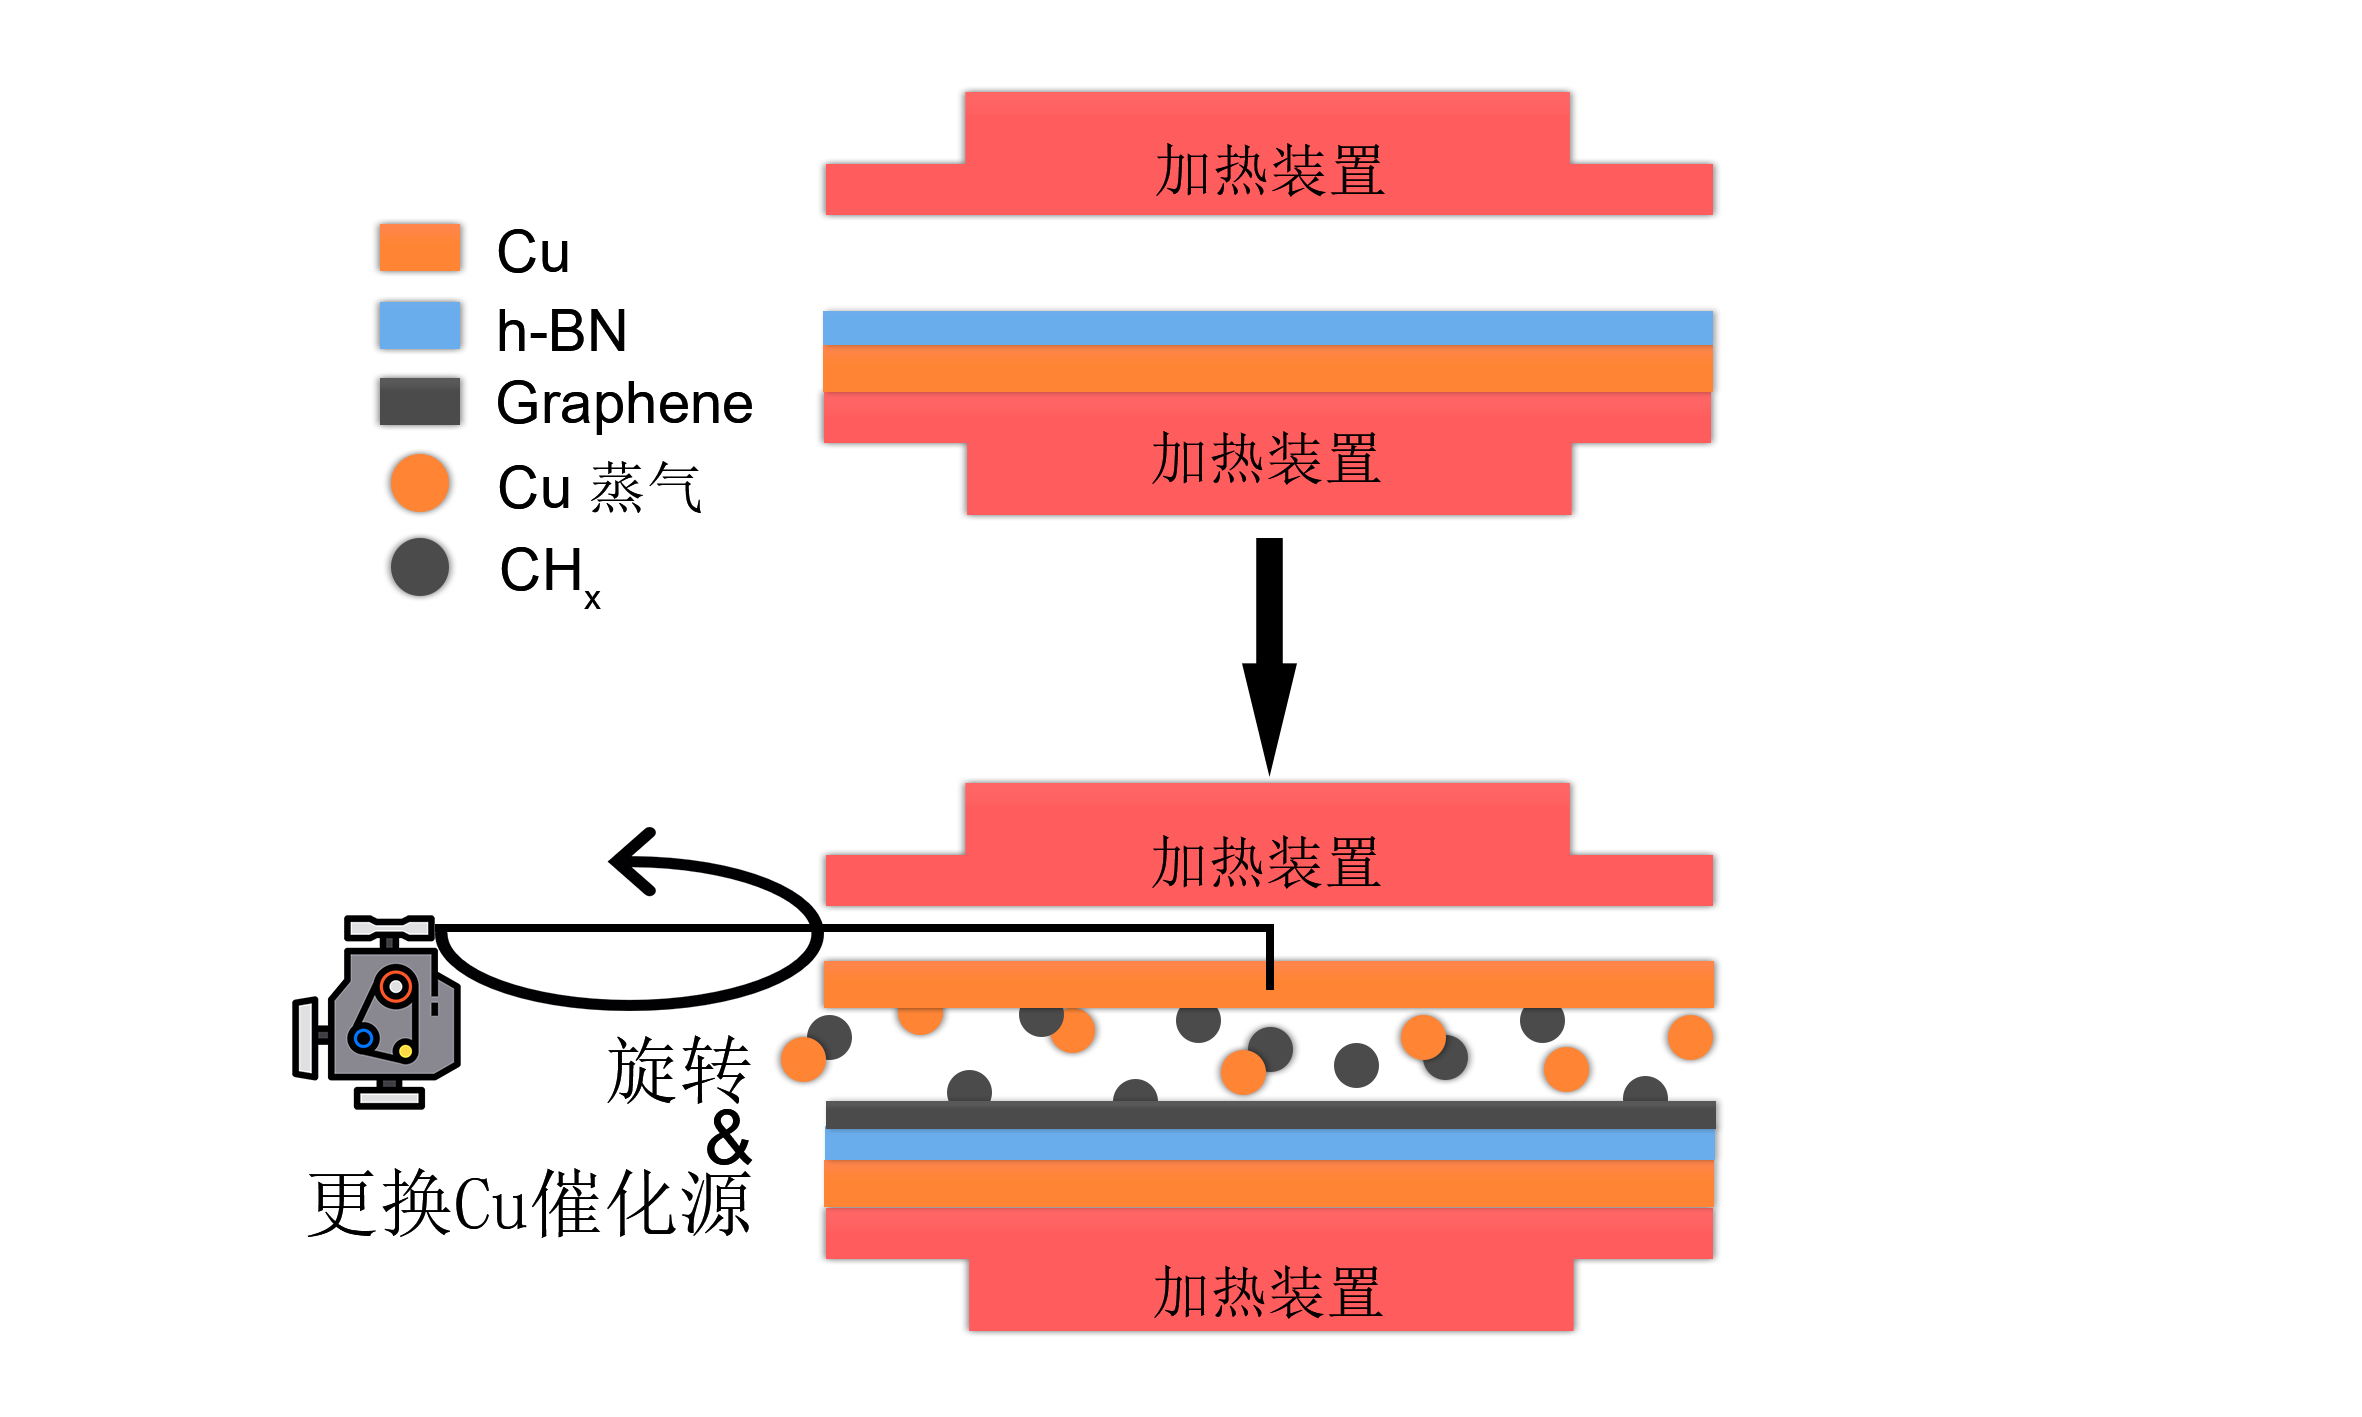
\includegraphics{pic/CG_diagram_routine.png}
            \label{fig:CG_diagram_routine}
        }\\[-0.5ex]
        \subfloat[]{
            \includegraphics{pic/CG_diagram_growthSketch.png}
            \label{fig:CG_diagram_growthSketch}
        }
        \caption{利用\cemb{Cu}蒸气近邻催化效应在\cemb{h-BN}表面直接堆叠生长石墨烯。(a)生长装置示意图;(b)石墨烯/\cemb{h-BN}异质结生长过程示意图。}
        \label{fig:CG_diagram_CVD}
    \end{figure}

    \subsection{近邻蒸发气态\cemb{Cu}催化剂的扩散}
    \label{CG:FEM_CuVapor}
    事实上,在\cemb{h-BN}上方的\cemb{Cu}蒸发源对于石墨烯在\cemb{h-BN}表面的直接石墨烯生长可能纯在两种作用\chinesecolon 一种是如上文所说的,\cemb{Cu}蒸发源的表面蒸发出浓度较高的\cemb{Cu}蒸气,这些\cemb{Cu}蒸气在扩散至\cemb{h-BN}表面仍然能够保持较高的浓度和分压。随后在\cemb{Cu}蒸气的催化作用下,生长气氛中的\cemb{CH4}逐渐脱氢裂解为活性碳原子\cemb{C},在\cemb{h-BN}表面成核生长成为石墨烯。另一种方式是\cemb{CH4}直接在\cemb{Cu}的表面脱氢裂解,产生的活性碳原子(\cemb{C})和活性碳氢化合物(\cemb{CH})等基团在热动能的作用下脱离\cemb{Cu}铜蒸发源的表面,扩散至下方\cemb{h-BN}的表面进行成核、生长石墨烯。

    为了判定并且验证在\cemb{h-BN}表面生长石墨烯的生长机制,我们首先使用自由分子流模拟\cemb{Cu}蒸发源产生的\cemb{Cu}蒸气在扩散至\cemb{h-BN}表面后的浓度。图\ref{fig:CG_diagram_FEM_structure}为我们所构建的在自由分子流模型下\cemb{Cu}蒸气产生和扩散的模拟结构图。我们考虑圆盘形的\cemb{Cu}衬底和\cemb{Cu}蒸发源,半径为\SI{500}{\micro\meter}。\cemb{Cu}蒸发源悬挂在\cemb{Cu}衬底和\cemb{h-BN}的上方,间隔一定距离。\cemb{Cu}蒸发源的温度设置为\SI{1200}{\kelvin},此时蒸发出的\cemb{Cu}蒸气的饱和蒸汽压约为\SI{1.25E-13}{\pascal}。对于蒸发出的\cemb{Cu}蒸气,我们只关注从蒸发源下表面蒸发出的\cemb{Cu}原子流,并且遵循朗缪尔蒸发公式(Langmuir’s Equation of evaporation)。
    
    \begin{figure}[htb]
        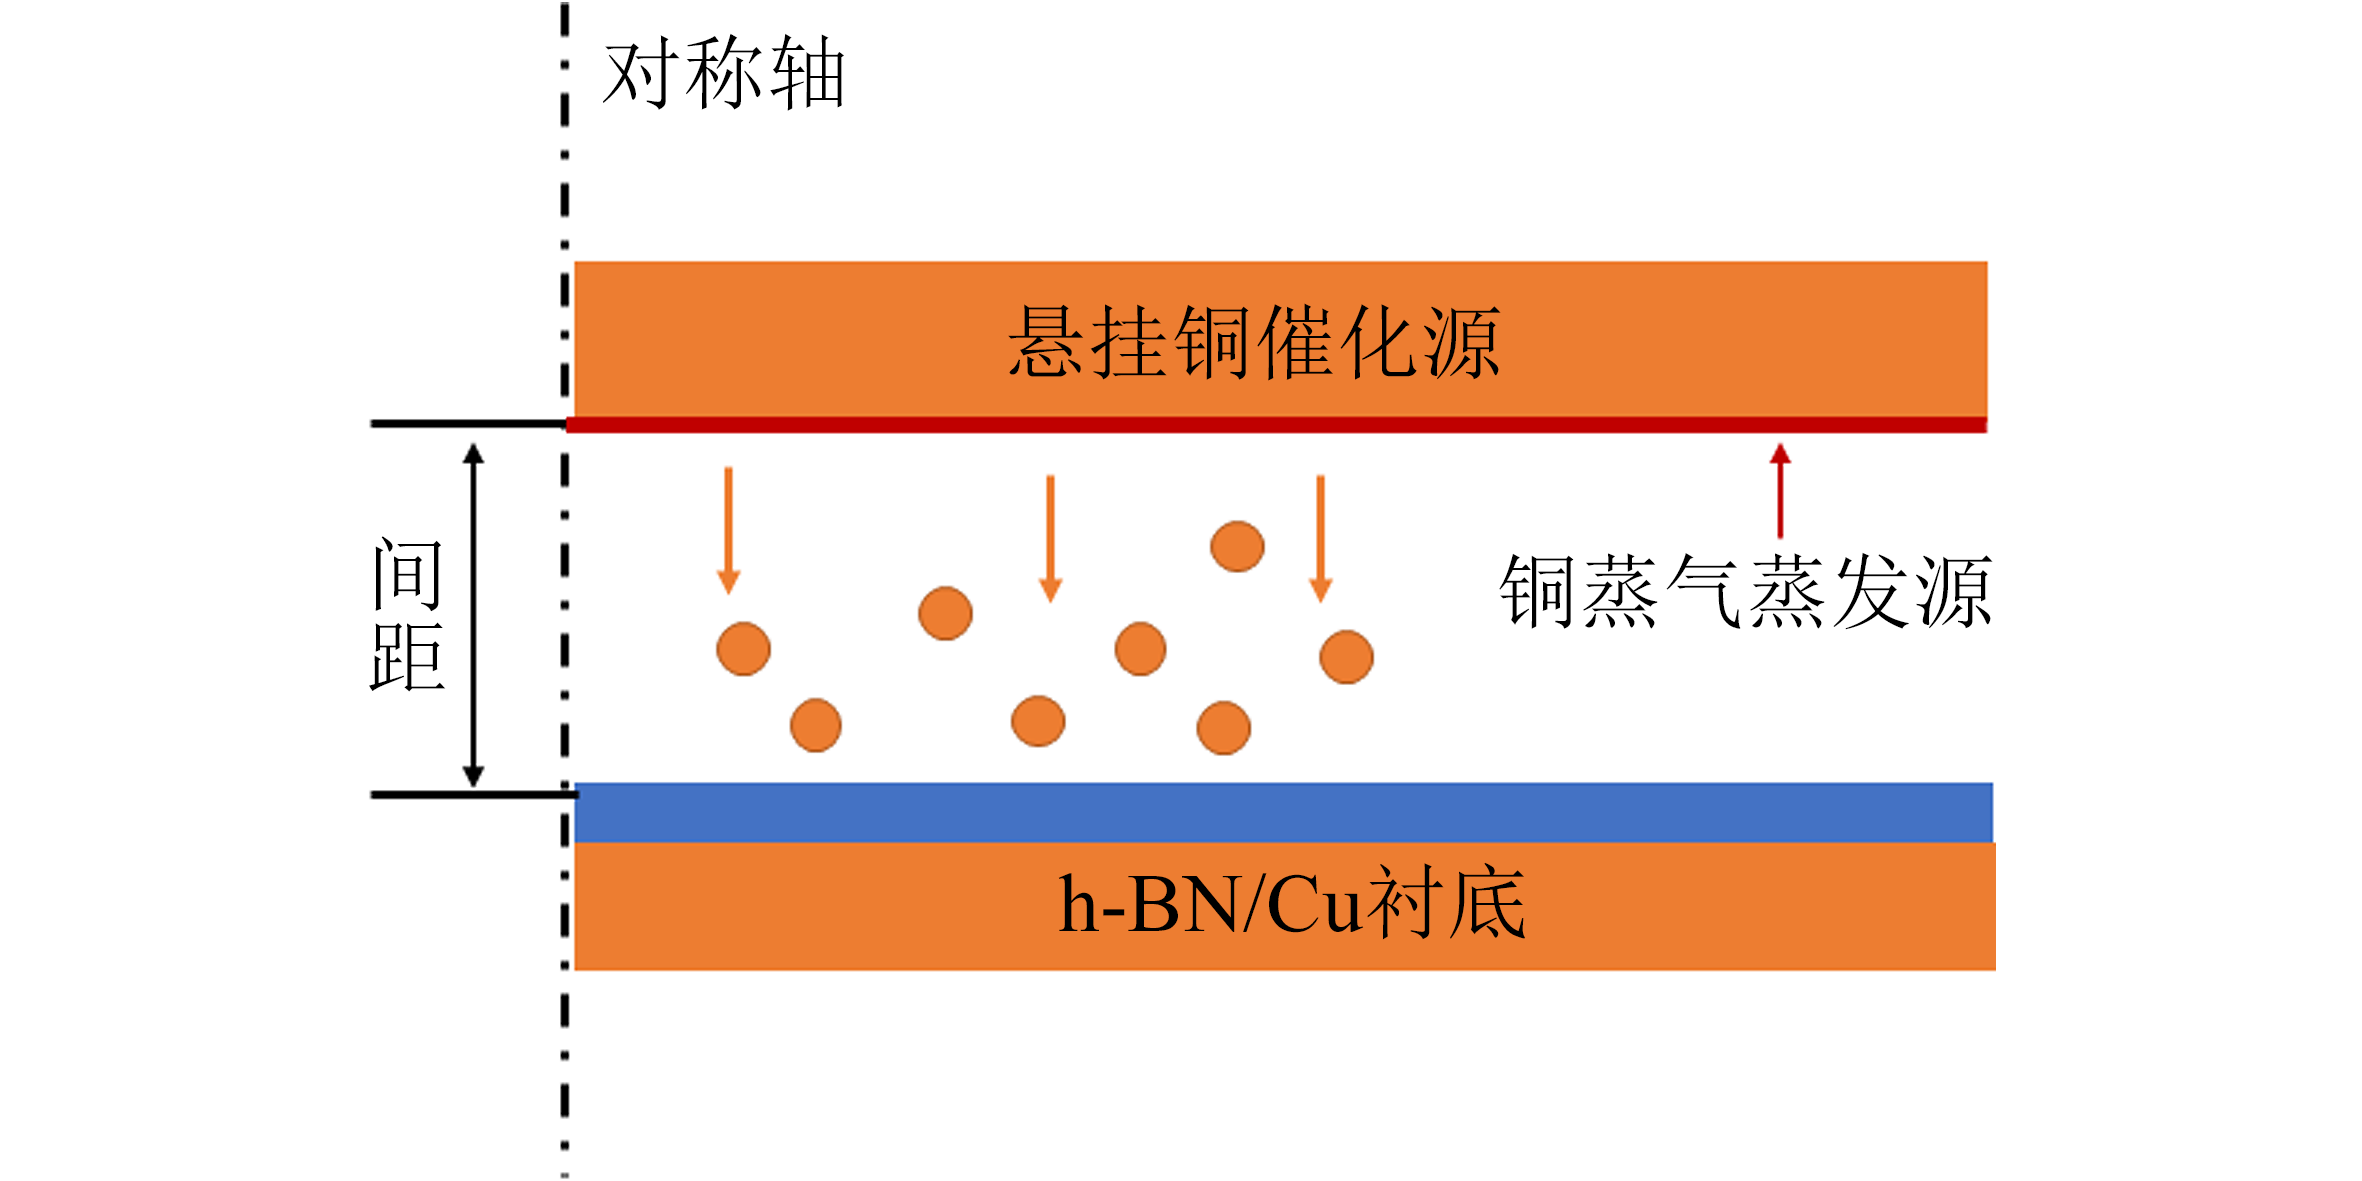
\includegraphics{pic/CG_diagram_FEM_structure.png}
        \caption{化学气相沉积腔体内\cemb{Cu}蒸气扩散模拟示意图。}
        \label{fig:CG_diagram_FEM_structure}
    \end{figure}

    使用自由分子流模拟,我们首先研究上方的\cemb{Cu}蒸发源未被石墨烯覆盖的情况。在图\ref{fig:CG_FEM_fullCu}中我们绘制了蒸发源和\cemb{Cu/h-BN}表面的距离在$\SI{4}{\micro\meter} \sim \SI{100}{\micro\meter}$的时候和,蒸发至下方\cemb{Cu/h-BN}表面的\cemb{Cu}蒸气的气压分布情况。可以看到对于\cemb{Cu/h-BN}表面,即使上方\cemb{Cu}蒸发源的距离从\SI{4}{\micro\meter}扩大至\SI{100}{\micro\meter}其的中心处的\cemb{Cu}蒸气的气压略微下降,接近于蒸发温度下的\cemb{Cu}原子的饱和蒸汽压\SI{1.25e-13}{\pascal}。当\cemb{Cu}蒸发源和\cemb{Cu/h-BN}之间的距离很近时,\cemb{Cu/h-BN}表面\cemb{Cu}蒸气的气压随着半径的衰减很小,只在接近边缘的位置由于\cemb{Cu}蒸气的向外扩散,导致\cemb{Cu/h-BN}表面边缘处(半径$\geqslant \SI{400}{\micro\meter}$)出现了\cemb{Cu}蒸气气压的明显下降。
    
    \begin{figure}[htb]
        \includegraphics{pic/CG_FEM_fullCu.png}
        \caption{不同间距下\cemb{Cu/h-BN}表面\cemb{Cu}蒸气的气压分布情况。}
        \label{fig:CG_FEM_fullCu}
    \end{figure}

    当\cemb{Cu}蒸发源和\cemb{Cu/h-BN}的距离扩大时,在\cemb{Cu/h-BN}表面\cemb{Cu}蒸气气压随着半径的衰减作用变强。当二者的距离提高到\SI{100}{\micro\meter}时,在\cemb{Cu/h-BN}表面半径为\SI{300}{\micro\meter}位置就已经可以观察到较为明显的\cemb{Cu}蒸气气压下降。当\cemb{Cu}蒸发源未被石墨烯覆盖的时候,在\cemb{Cu/h-BN}表面最外缘处(\SI{500}{\micro\meter})的\cemb{Cu}蒸气气压随与\cemb{Cu}蒸发源之间距离的上升而下降的驱使不明显。当距离为\SI{4}{\micro\meter}时,\cemb{Cu/h-BN}表面最外缘处的\cemb{Cu}蒸气气压为\SI{8e-4}{\pascal}。而当距离扩展到\SI{100}{\micro\meter}时,在\cemb{Cu/h-BN}表面最外缘处仍可以保持大约\SI{6e-4}{\pascal}的\cemb{Cu}蒸气。

    当在\cemb{Cu/h-BN}的表面生长了一段时间的石墨烯后,由于\cemb{CH4}在\cemb{Cu}蒸发源的表面同样会裂解沉积生长石墨烯,\cemb{Cu}蒸发源会有部分表面覆盖上新生长的石墨烯而从而失去蒸发\cemb{Cu}蒸气的能力。考虑到石墨烯生长前驱体\cemb{CH4}通常来自\cemb{Cu}蒸发源外部的气流,因此我们简单的将\cemb{Cu}蒸发源表面随着生长过程进行而生长的石墨烯限制在\cemb{Cu}蒸发源圆盘的外缘(半径$\geqslant \SI{250}{\micro\meter}$)。在图\ref{fig:CG_FEM_halfCu}中,我们模拟了在被石墨烯覆盖了外半圈\cemb{Cu}蒸发源的情况下,扩散至\cemb{Cu/h-BN}表面\cemb{Cu}蒸气的气压分布情况。可以看到相比于完整的\cemb{Cu}蒸发源,即使在\cemb{Cu}蒸发源和\cemb{Cu/h-BN}相距很近的情况下(\SI{4}{\micro\meter}),被石墨烯覆盖的\cemb{Cu}蒸发源只能在\cemb{Cu/h-BN}表面的正对于未被石墨烯覆盖的\cemb{Cu}蒸发源的位置维持较高压强的\cemb{Cu}铜蒸气(半径$\leqslant \SI{250}{\micro\meter}$)。
    同时,在这些正对于未被石墨烯覆盖的\cemb{Cu}蒸发源的位置,扩散至其上的\cemb{Cu}蒸气的浓度随着距离上升而下降的速度也略快于未被石墨烯覆盖时的情况。

    \begin{figure}[htb]
        \includegraphics{pic/CG_FEM_halfCu.png}
        \caption{不同间距下\cemb{Cu}蒸发源的外半圈被石墨烯覆盖后蒸发、扩散至\cemb{Cu/h-BN}表面的\cemb{Cu}蒸气的气压分布情况。}
        \label{fig:CG_FEM_halfCu}
    \end{figure}

    而在\cemb{Cu/h-BN}表面正对于上方被石墨烯覆盖的\cemb{Cu}蒸发源的位置,扩散至这些位置的\cemb{Cu}蒸气的浓度急剧下降。在模拟系统中\cemb{Cu/h-BN}表面的边缘(\SI{500}{\micro\meter}),\cemb{Cu}蒸气的浓度下降至约\SI{1e-4}{\pascal},远低于未被石墨烯覆盖时的\SI{6E-4}{\pascal}。值得注意的是,在\cemb{Cu/h-BN}边缘的位置,\cemb{Cu}蒸发源和\cemb{Cu/h-BN}距离较远时\cemb{Cu}蒸气的浓度反超了距离较近时的情况(半径$\geqslant \SI{450}{\micro\meter}$)。这是由于在与\cemb{Cu}蒸发源的距离较远时,\cemb{Cu/h-BN}表面边缘能够更好的接收到来自\cemb{Cu}蒸发源中央的\cemb{Cu}蒸气原子,而这些原子在距离较近时会直接扩散至\cemb{Cu/h-BN}表面中央的区域。
    因此,悬挂的\cemb{Cu}蒸发源需要在生长过程中经常性得进行更换,以保持较为完整的\cemb{Cu}表面,防止石墨烯覆盖后对\cemb{Cu}蒸气扩散至下方\cemb{Cu/h-BN}表面的\cemb{Cu}蒸气的浓度和均匀度产生影响,最终导致在\cemb{Cu/h-BN}表面石墨烯生长速度减慢以及生长均匀性变差的情况。

    考虑到在实际的生长过程中,用于提供\cemb{Cu}蒸气的\cemb{Cu}蒸发源可以比生长区域大得多(尺寸在\si{\centi\meter}级),因此我们可以利用模拟\cemb{Cu/h-BN}中心处的\cemb{Cu}蒸气气压来代表生长区域中参与近邻催化裂解\cemb{CH4}的\cemb{Cu}蒸气气压。在图\ref{fig:CG_FEM_fullCuCenterVariousDistance}中,我们计算了\cemb{Cu}蒸发源和\cemb{Cu/h-BN}距离从微米级\si{\micro\meter}扩大至厘米级\si{\milli\meter}时,在石墨烯生长区域中\cemb{Cu}蒸气的气压变化情况。我们可以看到当距离小于\SI{1}{\milli\meter}(\SI{1000}{\micro\meter})时,从\cemb{Cu}蒸发源蒸发、扩散至\cemb{Cu/h-BN}表面的\cemb{Cu}蒸气的气压变化较小,且非常接近于\cemb{Cu}原子的饱和蒸汽压\SI{1.25e-13}。而当二者之间的距离继续增,\cemb{Cu}蒸气的压强极速下降。距离为\SI{10}{\milli\meter}(\SI{10000}{\micro\meter})时,模拟得到的在\cemb{Cu/h-BN}表面的\cemb{Cu}蒸气的气压仅有约\SI{4e-4}{\pascal}。\cemb{Cu/h-BN}表面的\cemb{Cu}蒸气气压随距离的变化与实验中的现象一致。
    %TODO 引用
    随着\cemb{Cu}蒸发源和\cemb{Cu/h-BN}表面之间的距离由\SI{10}{\micro\meter}增长至\SI{1}{\milli\meter}和\SI{10}{\milli\meter},在\cemb{Cu/h-BN}表面直接生长的石墨烯的覆盖率也随之减少。

    \begin{figure}[htb]
        \includegraphics{pic/CG_FEM_fullCuCenterVariousDistance.png}
        \caption{不同间距下从\cemb{Cu}蒸发源蒸发、扩散至\cemb{Cu/h-BN}表面中央的\cemb{Cu}蒸气的气压情况。}
        \label{fig:CG_FEM_fullCuCenterVariousDistance}
    \end{figure}

    另一方面,考虑到在温度为\SI{1300}{\kelvin}时,石墨碳的饱和蒸汽压仅有\SI{1e-17}{\pascal}\citing{RN788-2004}。因此我们认为相比于从扩散而来的\cemb{C}、\cemb{CH},在\cemb{Cu/h-BN}表面直接堆叠生长的石墨烯更可能来源于前驱体\cemb{CH4}利用\cemb{Cu}蒸气的近邻催化作用在\cemb{Cu/h-BN}表面裂解而产生的\cemb{C}、\cemb{CH}等活性碳化物。

    \subsection{气态\cemb{Cu}催化剂对甲烷裂解反应的催化性能}
    在\ref{CG:FEM_CuVapor}章中,我们证明了当\cemb{Cu}蒸发源和\cemb{Cu/h-BN}衬底的距离足够近时,能够有足够的\cemb{Cu}蒸气扩散至\cemb{h-BN}的表面进行\cemb{CH4}裂解的催化作用。接下来我们利用密度泛函理论计算,探究\cemb{Cu}蒸气对于\cemb{CH4}脱氢裂解反应的催化作用。在计算中,我们使用包含1~3个原子的\cemb{Cu}团簇(\cemb{Cu}、\cemb{Cu2}、\cemb{Cu3})代表\cemb{Cu}蒸气中的气态物质。\cemb{Cu}蒸气对于\cemb{CH4}裂解反应的催化能力通过考察\cemb{CH4}在不同\cemb{Cu}团簇表面的脱氢反应的激活能进行标定。在本章的激活能计算中,我们考虑\cemb{CH4}脱氢的四步脱氢基元反应,每步反应都从吸附在\cemb{Cu}团簇上的\cemb{CH4}分子中脱出一个\cemb{H}原子\chinesecolon
    \begin{equation}
        \label{chemeq:CH4deH}
        \begin{split}
            \cemb{CH4 &-> CH3 + H}\\
            \cemb{CH3 &-> CH2 + H}\\
            \cemb{CH2 &-> CH + H}\\
            \cemb{CH &-> C + H}
        \end{split}
    \end{equation}

    经过四步脱氢反应后,生长气氛中的\cemb{CH4}分子转变为活性的\cemb{C}原子,\cemb{C}原子在\cemb{Cu/h-BN}的表面作为碳源直接参与石墨烯的堆叠生长。如图\ref{fig:CG_DFT_CuCHx}所示,利用密度泛函理论方法,我们计算了在不同\cemb{Cu}团簇的表面,\cemb{CH4}四步脱氢裂解反应的反应激活能和反应能的变化情况。在图\ref{fig:CG_DFT_CuCHx}中,我们额外给出了无催化剂的参与下\cemb{CH4}脱氢裂解反应的能量变化曲线作为参考。

        \begin{figure}[!htb]
        \includegraphics{pic/CG_DFT_CuCHx.png}
        \caption{\cemb{CH4}在\cemb{Cu}、\cemb{Cu2}、\cemb{Cu3}团簇以及无催化剂表面脱氢裂解的反应能和反应激活能变化情况。其中TS代表反应过渡态,其值为反应所需的激活能大小。在原子结构中,铜原子为橙色;碳原子为灰色;氢原子为白色。}
        \label{fig:CG_DFT_CuCHx}
    \end{figure}

    可以看到,在没有\cemb{Cu}等催化剂的介入下\cemb{CH4}脱氢每步大约需要$\SI{3.69}{\electronvolt}\sim  \SI{4.9}{\electronvolt}$的激活能。如此高的反应激活需求使得反应气氛中的\cemb{CH4}难以直接裂解为\cemb{C}、\cemb{CH}等活性基团以供石墨烯的生长。当\cemb{Cu}团簇被引入作为催化剂后,密度泛函理论计算得到的\cemb{CH4}脱氢反应的激活能相比于无催化剂的情况产生了大幅度的下降。四步脱氢反应的激活能由无催化剂的最高约\SI{4.9}{\electronvolt}下降至\cemb{Cu}团簇作为催化剂的最高约\SI{2.7}{\electronvolt}。同时我们还可以发现,随着\cemb{Cu}团簇内包含的\cemb{Cu}原子的数目上升,\cemb{CH4}脱氢裂解反应的激活能和反应能由逐渐下降的趋势。

    通过和无催化剂辅助情况下\cemb{CH4}脱氢裂解的激活能和反应能进行比较,我们可以认为\cemb{Cu}团簇能够使\cemb{CH4}的脱氢裂解反应能量需求大幅下降。在表\ref{tab:CH4_cata}中,我们将\cemb{CH4}在\cemb{Cu}团簇表面和在平坦的\cemb{Cu(111)}衬底表面催化裂解过程的反应激活能($\energyVar{a}{}$)和反应能$\Delta \energyVar{}{}$进行对比,探究\cemb{Cu}团簇的催化能力是否能够支撑石墨烯的生长。

    \begin{table}[htb]
    \def\aColWidth{0.20\textwidth}
    \def\bColWidth{0.10\textwidth}
    \def\cColWidth{0.12\textwidth}
    \def\dColWidth{0.12\textwidth}
    \def\eColWidth{0.12\textwidth}
    \def\fColWidth{0.12\textwidth}
    \def\abColwidth{0.3\textwidth}
    \caption{\cemb{Cu}团簇和\cemb{Cu(111)}衬底表面\cemb{CH4}脱氢裂解反应的激活能$\energyVar{a}{}$和反应能$\Delta\energyVar{}{}$}
    \label{tab:CH4_cata}
    \begin{tabular}{
        m{\aColWidth}
        >{\centering}m{\bColWidth}
        >{\centering}m{\cColWidth}
        >{\centering}m{\dColWidth}
        >{\centering}m{\eColWidth}
        >{\centering\arraybackslash}m{\fColWidth}
    }
    \toprule
    \multicolumn{2}{c}{\multirow{3.5}{*}{反应步骤}}&\multicolumn{3}{c}{\cemb{Cu}团簇构型}&\cemb{Cu}衬底表面\\
    \cmidrule{3-6}
    &&\cemb{Cu}团簇&\cemb{Cu2}团簇&\cemb{Cu3}团簇&\cemb{Cu(111)}表面\citing{RN789-2013}\\
    \midrule
    \multirow{2}{\abColwidth}{\cemb{CH4 -> CH3 + H}} & $\energyVar{a}{}\ \ (\si{\electronvolt})$&1.51&1.57&0.92&1.88\\
    &$\Delta \energyVar{}{}\;(\si{\electronvolt})$&0.43&0.35&0.05&0.86\\
    \multirow{2}{\abColwidth}{\cemb{CH3 -> CH2 + H}} &$\energyVar{a}{}\ \ (\si{\electronvolt})$&2.52&1.61&1.54&1.47\\
    &$\Delta \energyVar{}{}\;(\si{\electronvolt})$&2.34&0.76&1.53&1.05\\
    \multirow{2}{\abColwidth}{\cemb{CH2 -> CH + H}} &$\energyVar{a}{}\ \ (\si{\electronvolt})$&2.37&2.70&1.53&1.05\\
    &$\Delta \energyVar{}{}\;(\si{\electronvolt})$&2.15&2.70&1.05&0.32\\
    \multirow{2}{\abColwidth}{\cemb{CH -> C + H}} &$\energyVar{a}{}\ \ (\si{\electronvolt})$&2.25&1.53&1.23&2.21\\
    &$\Delta \energyVar{}{}\;(\si{\electronvolt})$&2.25&1.38&1.23&1.20\\
    \midrule
    \multirow{2}{\abColwidth}{\shortstack{总反应\\\cemb{CH4 -> C + 4H}}}&$\energyVar{a}{}\ \ (\si{\electronvolt})$&2.52&2.70&1.54&2.21\\
    &$\Delta \energyVar{}{}\;(\si{\electronvolt})$&7.17&5.19&3.09&3.08\\
    \bottomrule
    \end{tabular}
\end{table}

    从激活能$\energyVar{a}{}$的计算分布来看\cemb{CH3 -> CH2 + H}为\cemb{CH4}的脱氢裂解反应在\cemb{Cu}团簇和\cemb{Cu3}团簇表面的决速步,需要分别翻越\SI{2.52}{\electronvolt}和\SI{1.53}{\electronvolt}的能量。对于\cemb{CH4}在\cemb{Cu2}表面的脱氢催化反应,激活能最大的脱氢步骤为\cemb{CH2 -> CH + H},此步的激活能为\SI{2.70}{\electronvolt}。在我们所计算的代表\cemb{Cu}蒸气的三种\cemb{Cu}团簇中,\cemb{Cu3}团簇的激活能低于\cemb{CH4}在\cemb{Cu}衬底表面脱氢裂解的激活能\SI{2.21}{\electronvolt}。在\cemb{Cu(001)}衬底的表面\cemb{CH4}裂解的决速步为最后一步\cemb{CH -> C + H}。因此相比于直接提供\cemb{C}原子,在\cemb{Cu(111)}衬底的表面\cemb{CH4}的脱氢裂解还能提供大量的\cemb{CH}基团进行石墨烯的成核生长。而在\cemb{Cu3}团簇的表面,由\cemb{CH4 -> CH + 3H}生成\cemb{CH}集团的反应过程的所需的最高激活能$\energyVar{a}{}=\SI{1.54}{\electronvolt}$,仅仅比\cemb{Cu(111)}表面同样生成\cemb{CH}的反应激活能(\SI{1.47}{\electronvolt})高\SI{0.07}{\electronvolt}。因此我们可以认为在\cemb{Cu3}团簇的表面,\cemb{CH4}裂解生成\cemb{CH}的的能力仅稍逊与\cemb{Cu(111)}的表面,同样能够提供大量的\cemb{CH}用于石墨烯在\cemb{Cu/h-BN}表面的直接成核生长。 

    进一步考虑\cemb{CH4}脱氢裂解的反应能情况。在\cemb{Cu}团簇的表面,\cemb{CH4}裂解的总应能随着团簇内包含\cemb{Cu}数量的上升由在\cemb{Cu}表面的\SI{7.17}{\electronvolt}下降至在\cemb{Cu3}表面的\SI{3.09}{\electronvolt},接近于在\cemb{Cu(111)}表面的\SI{3.08}{\electronvolt}的反应吸热。更低的反应能意味着有更多的\cemb{CH4}在热动能的推动下转化为\cemb{C},为\cemb{Cu/h-BN}表面生长的石墨烯提供更为充足的碳源。
    
    \begin{figure}[!htb]
        \subfloat[]{
            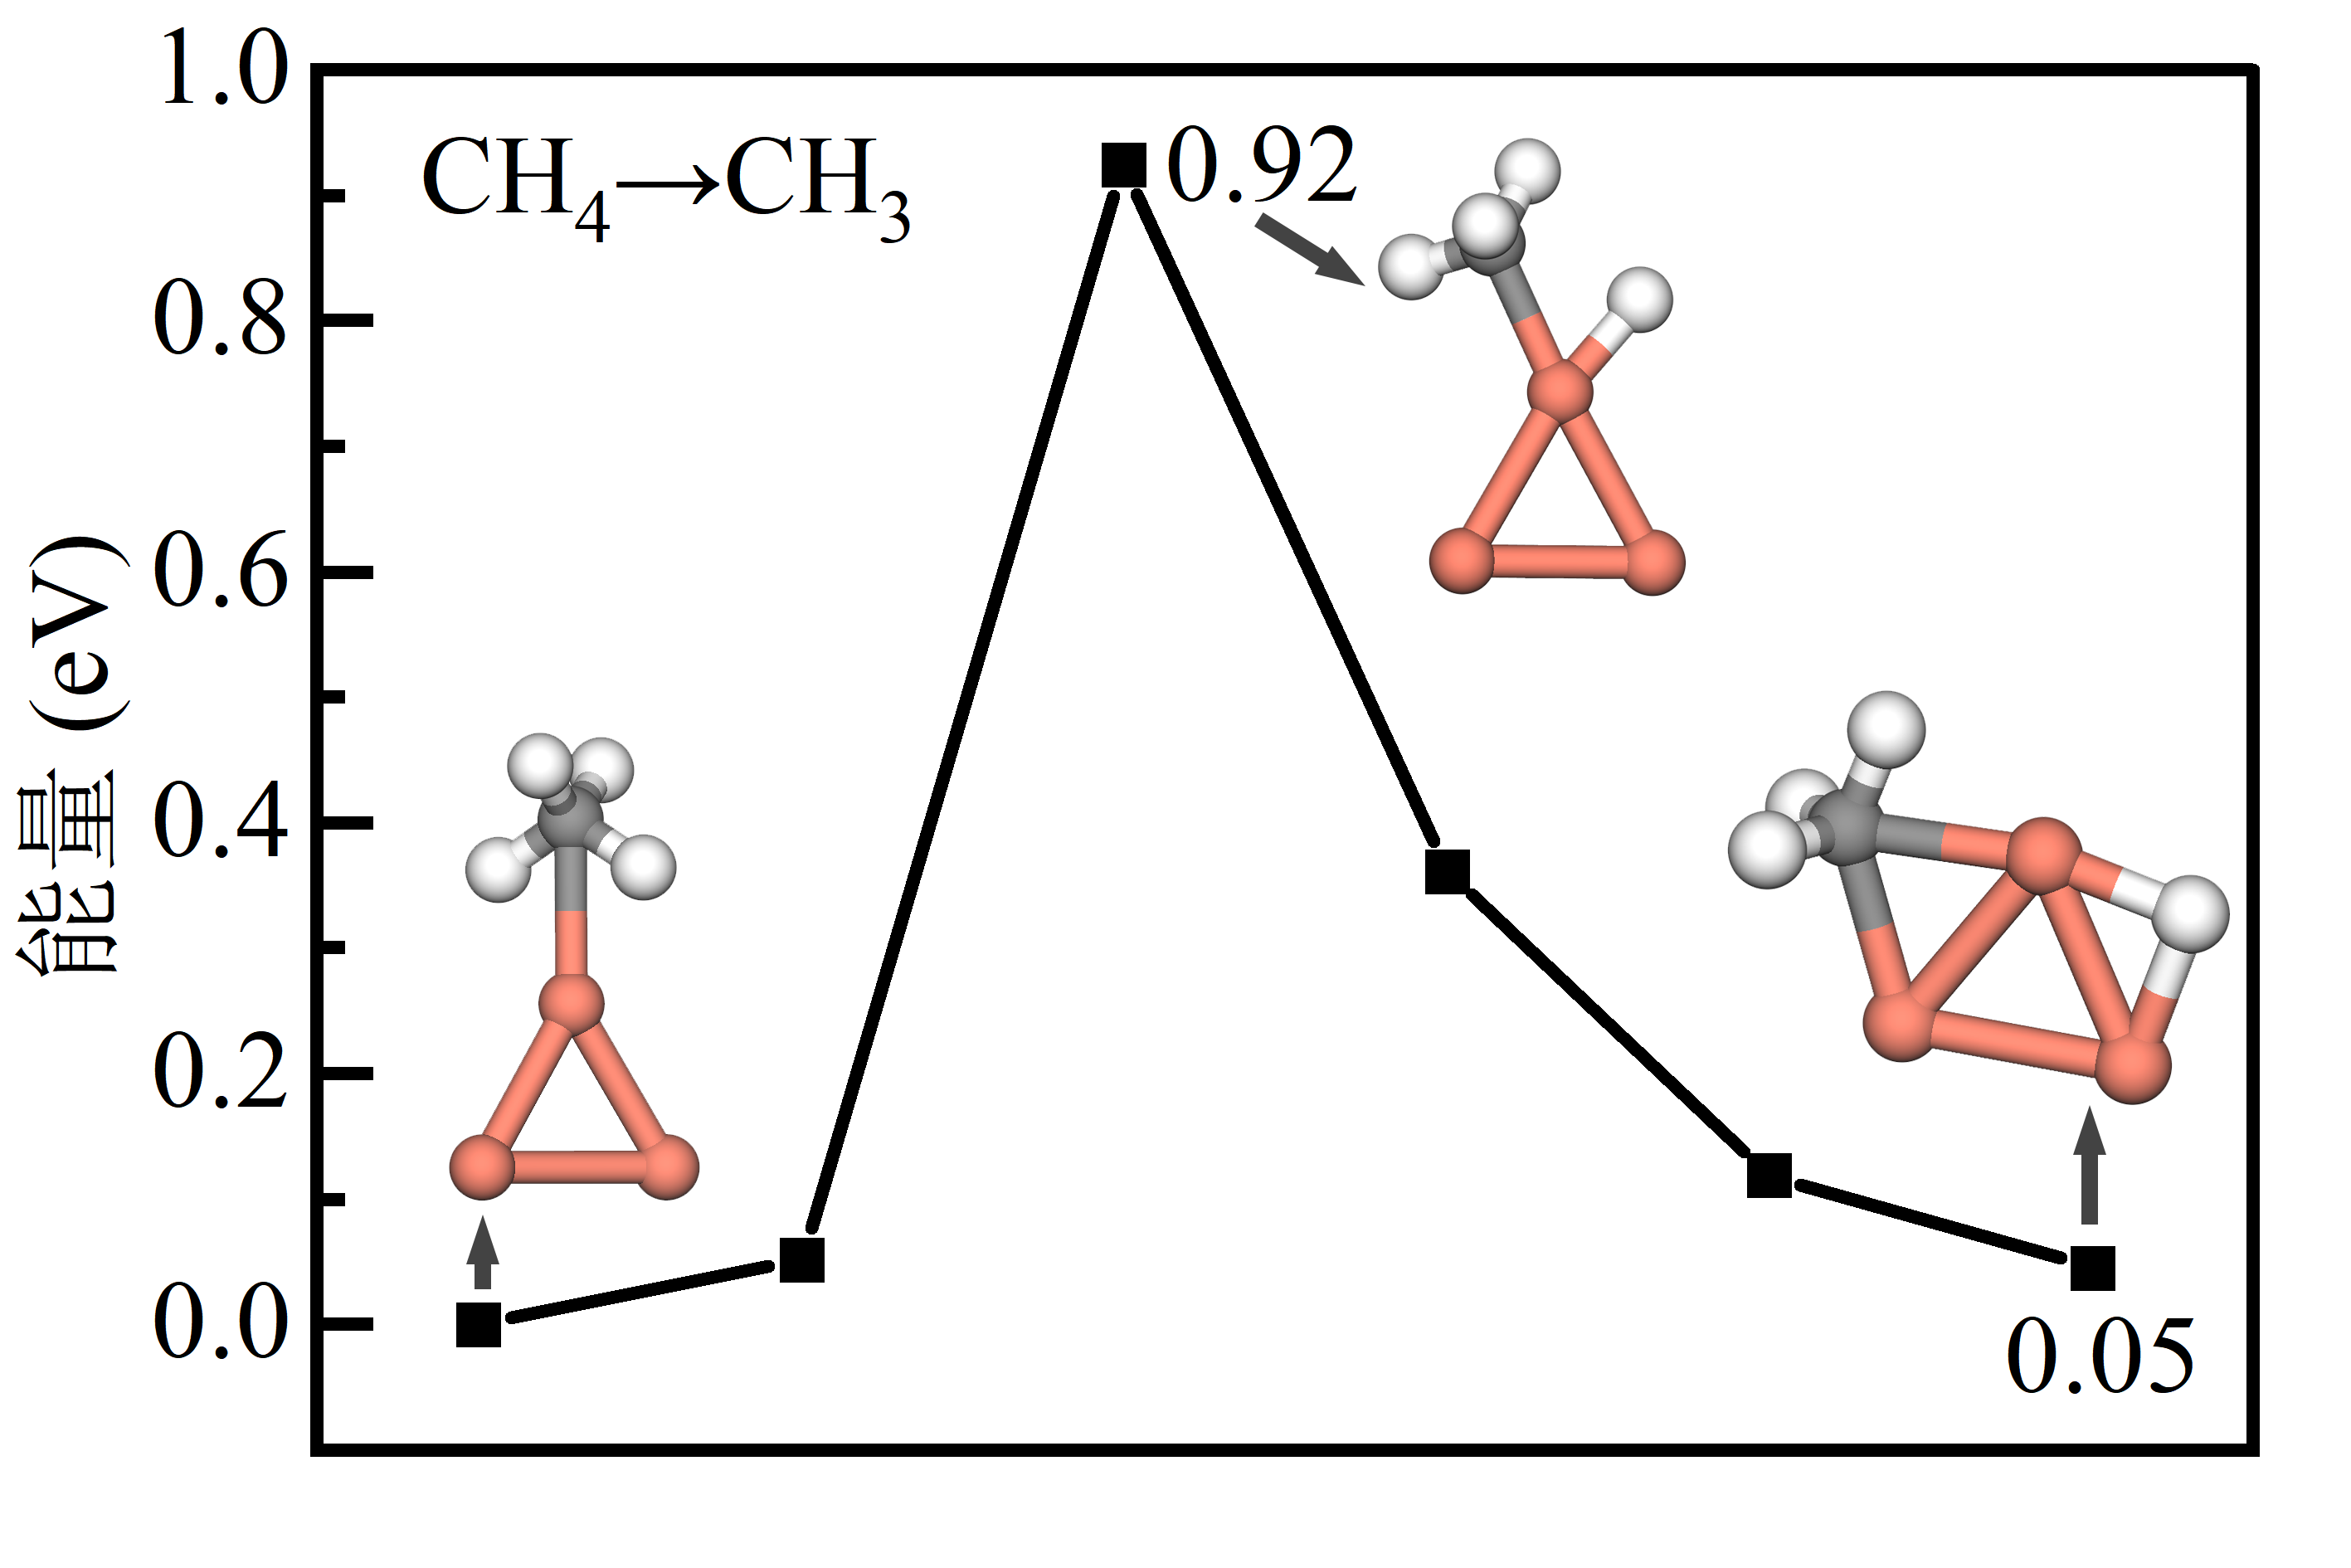
\includegraphics[width=0.45\textwidth]{pic/CG_DFT_Cu3-CH4-CH3.png}
        }
        \subfloat[]{
            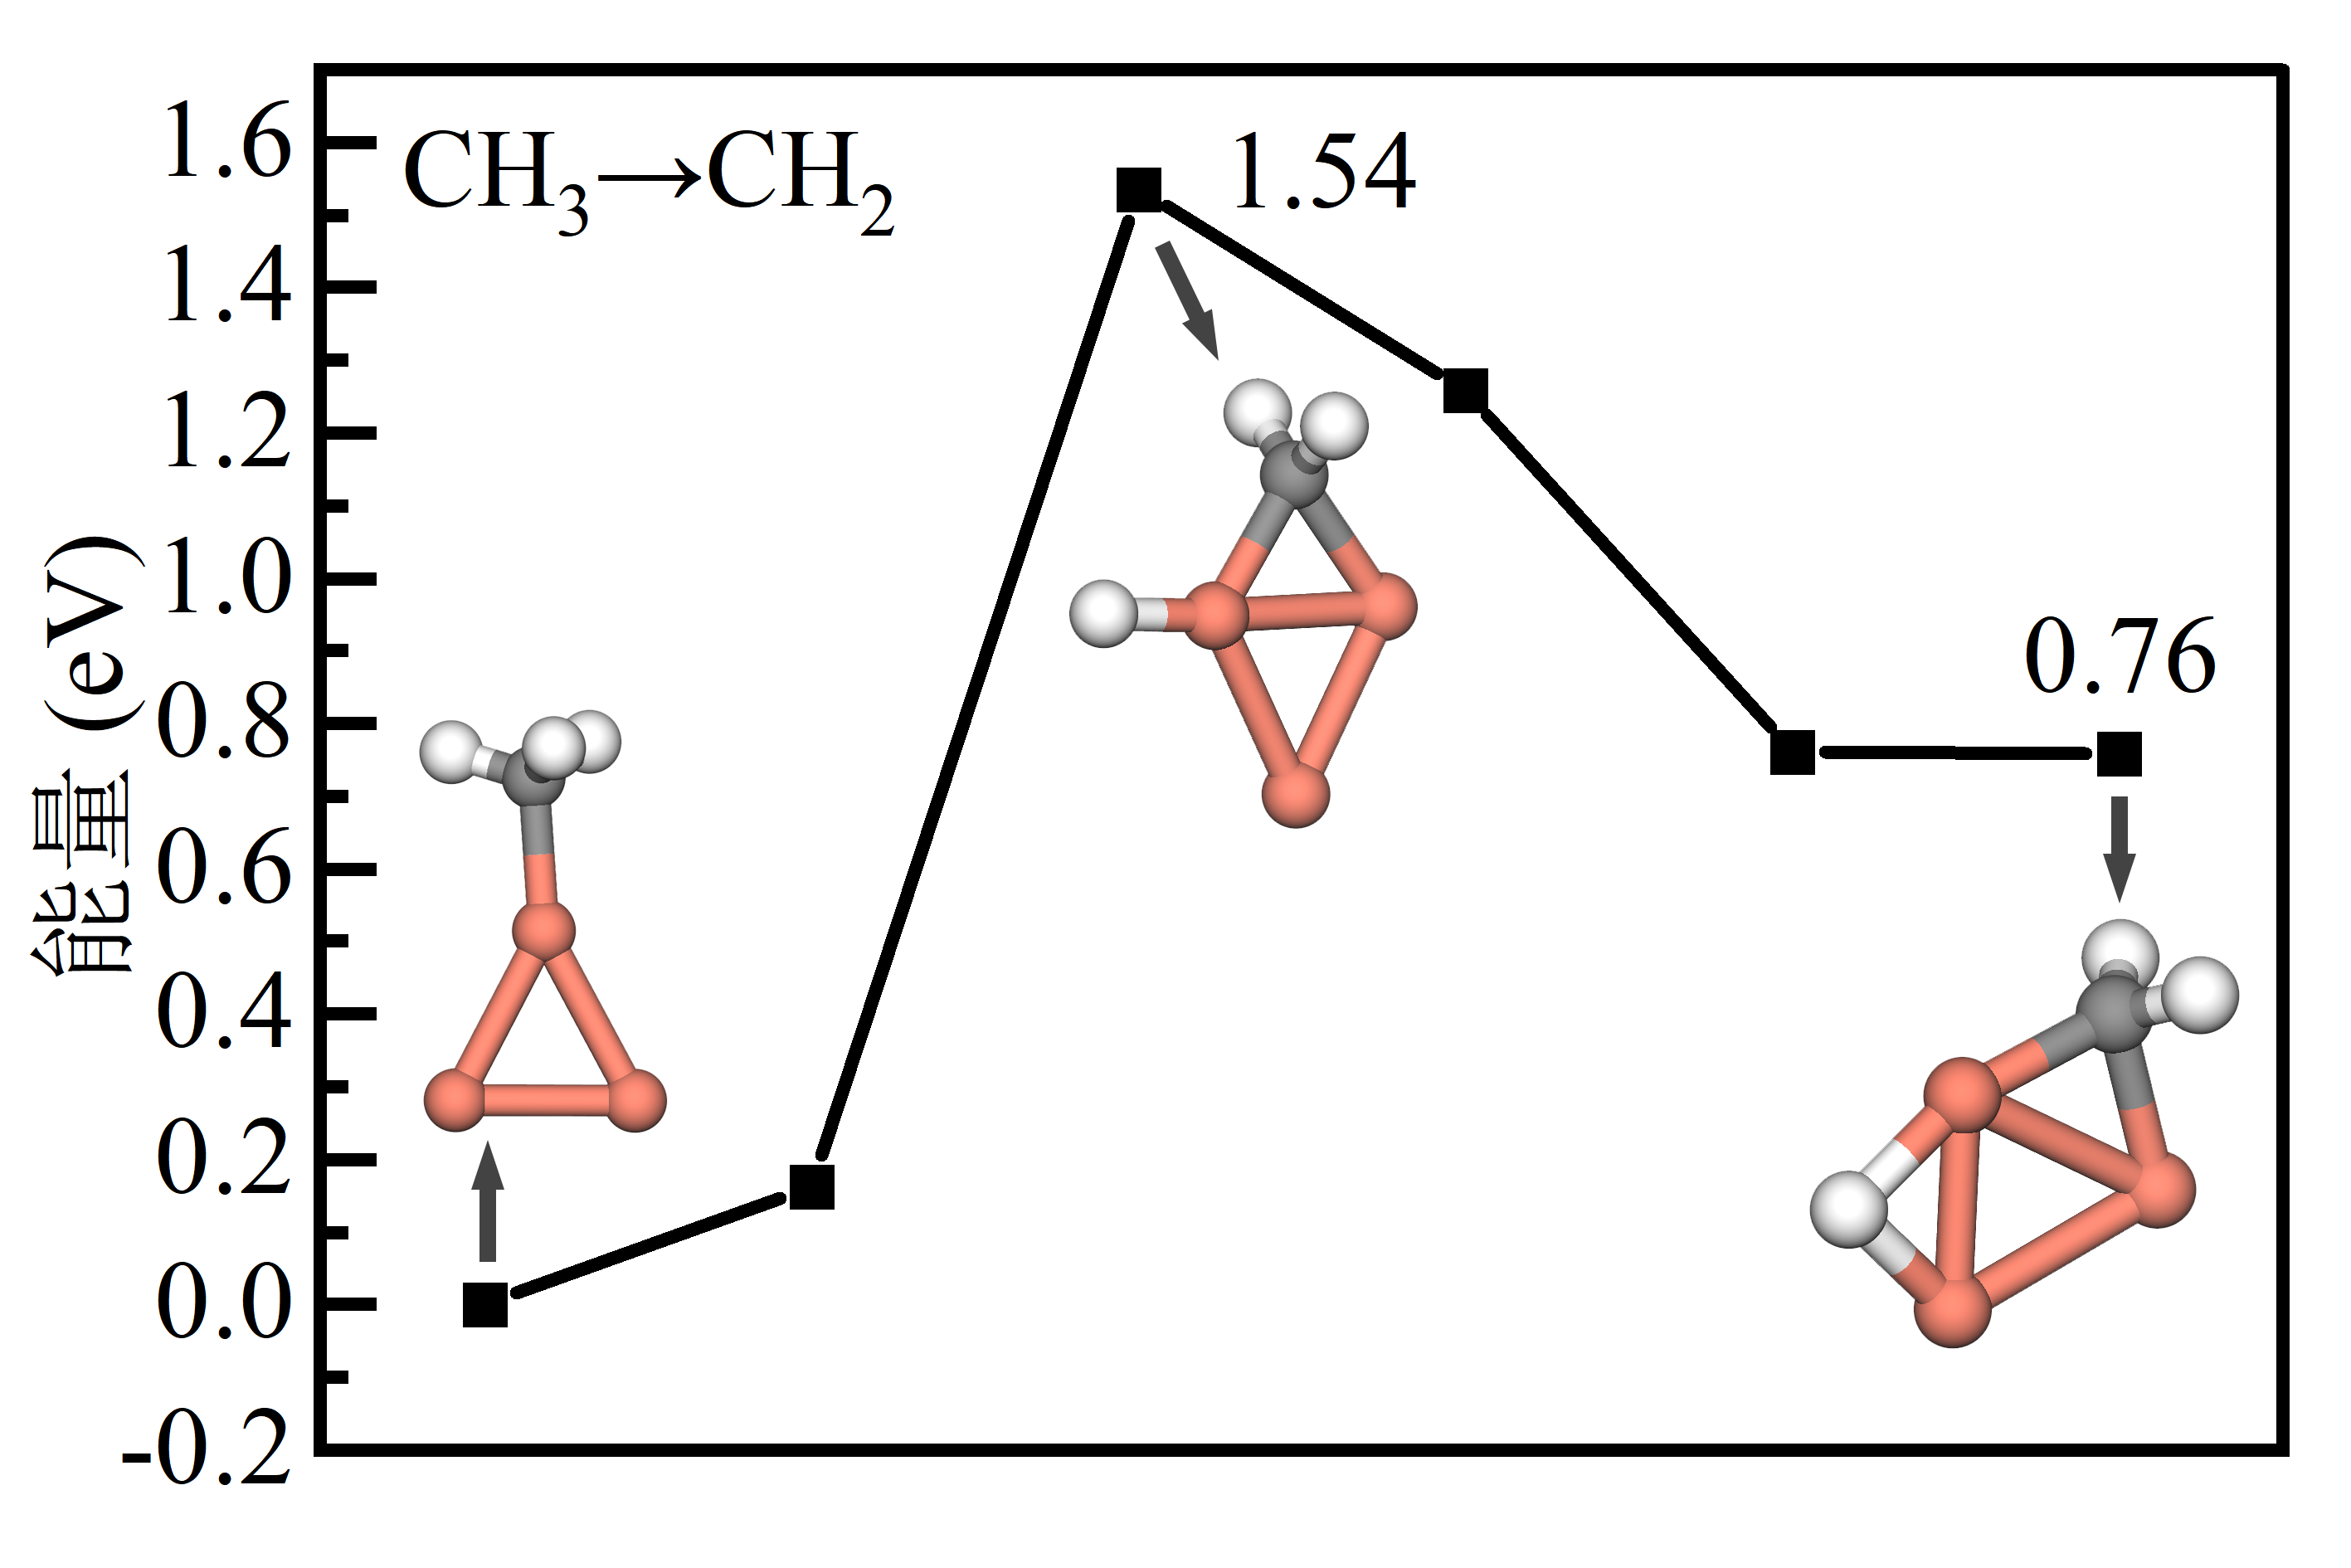
\includegraphics[width=0.45\textwidth]{pic/CG_DFT_Cu3-CH3-CH2.png}
        }\\[-0.5ex]
        \subfloat[]{
            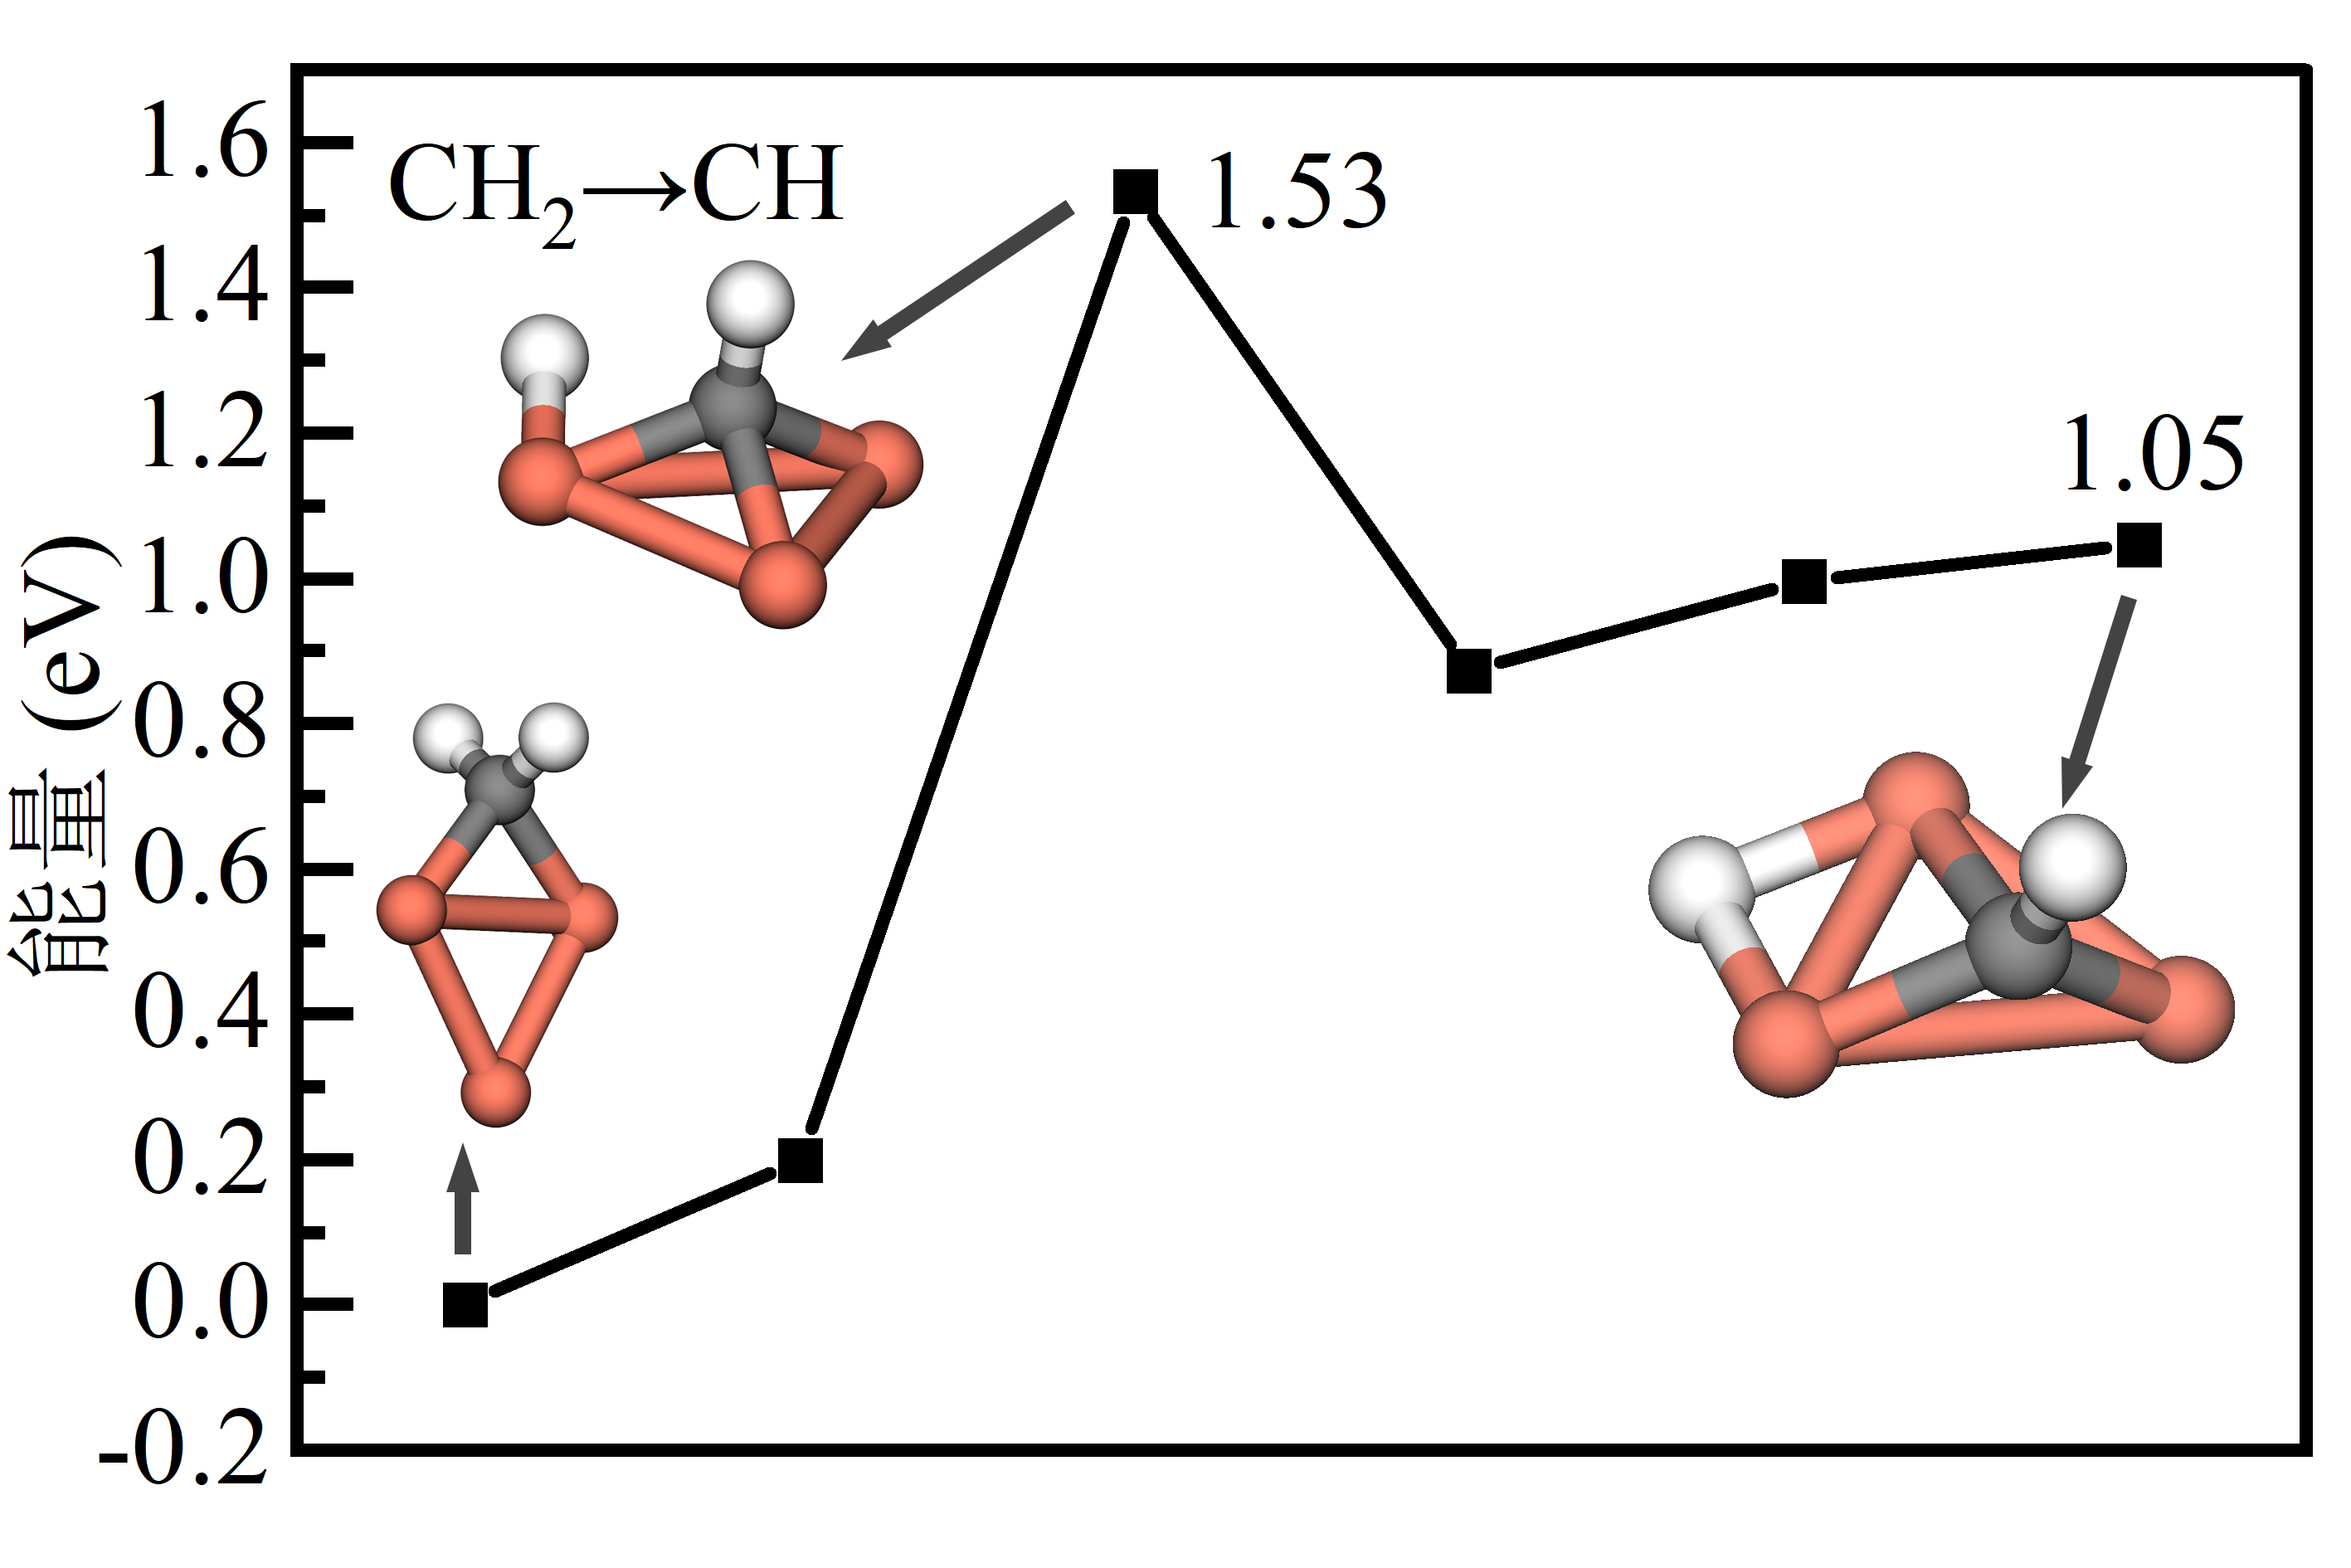
\includegraphics[width=0.45\textwidth]{pic/CG_DFT_Cu3-CH2-CH.png}
        }
        \subfloat[]{
            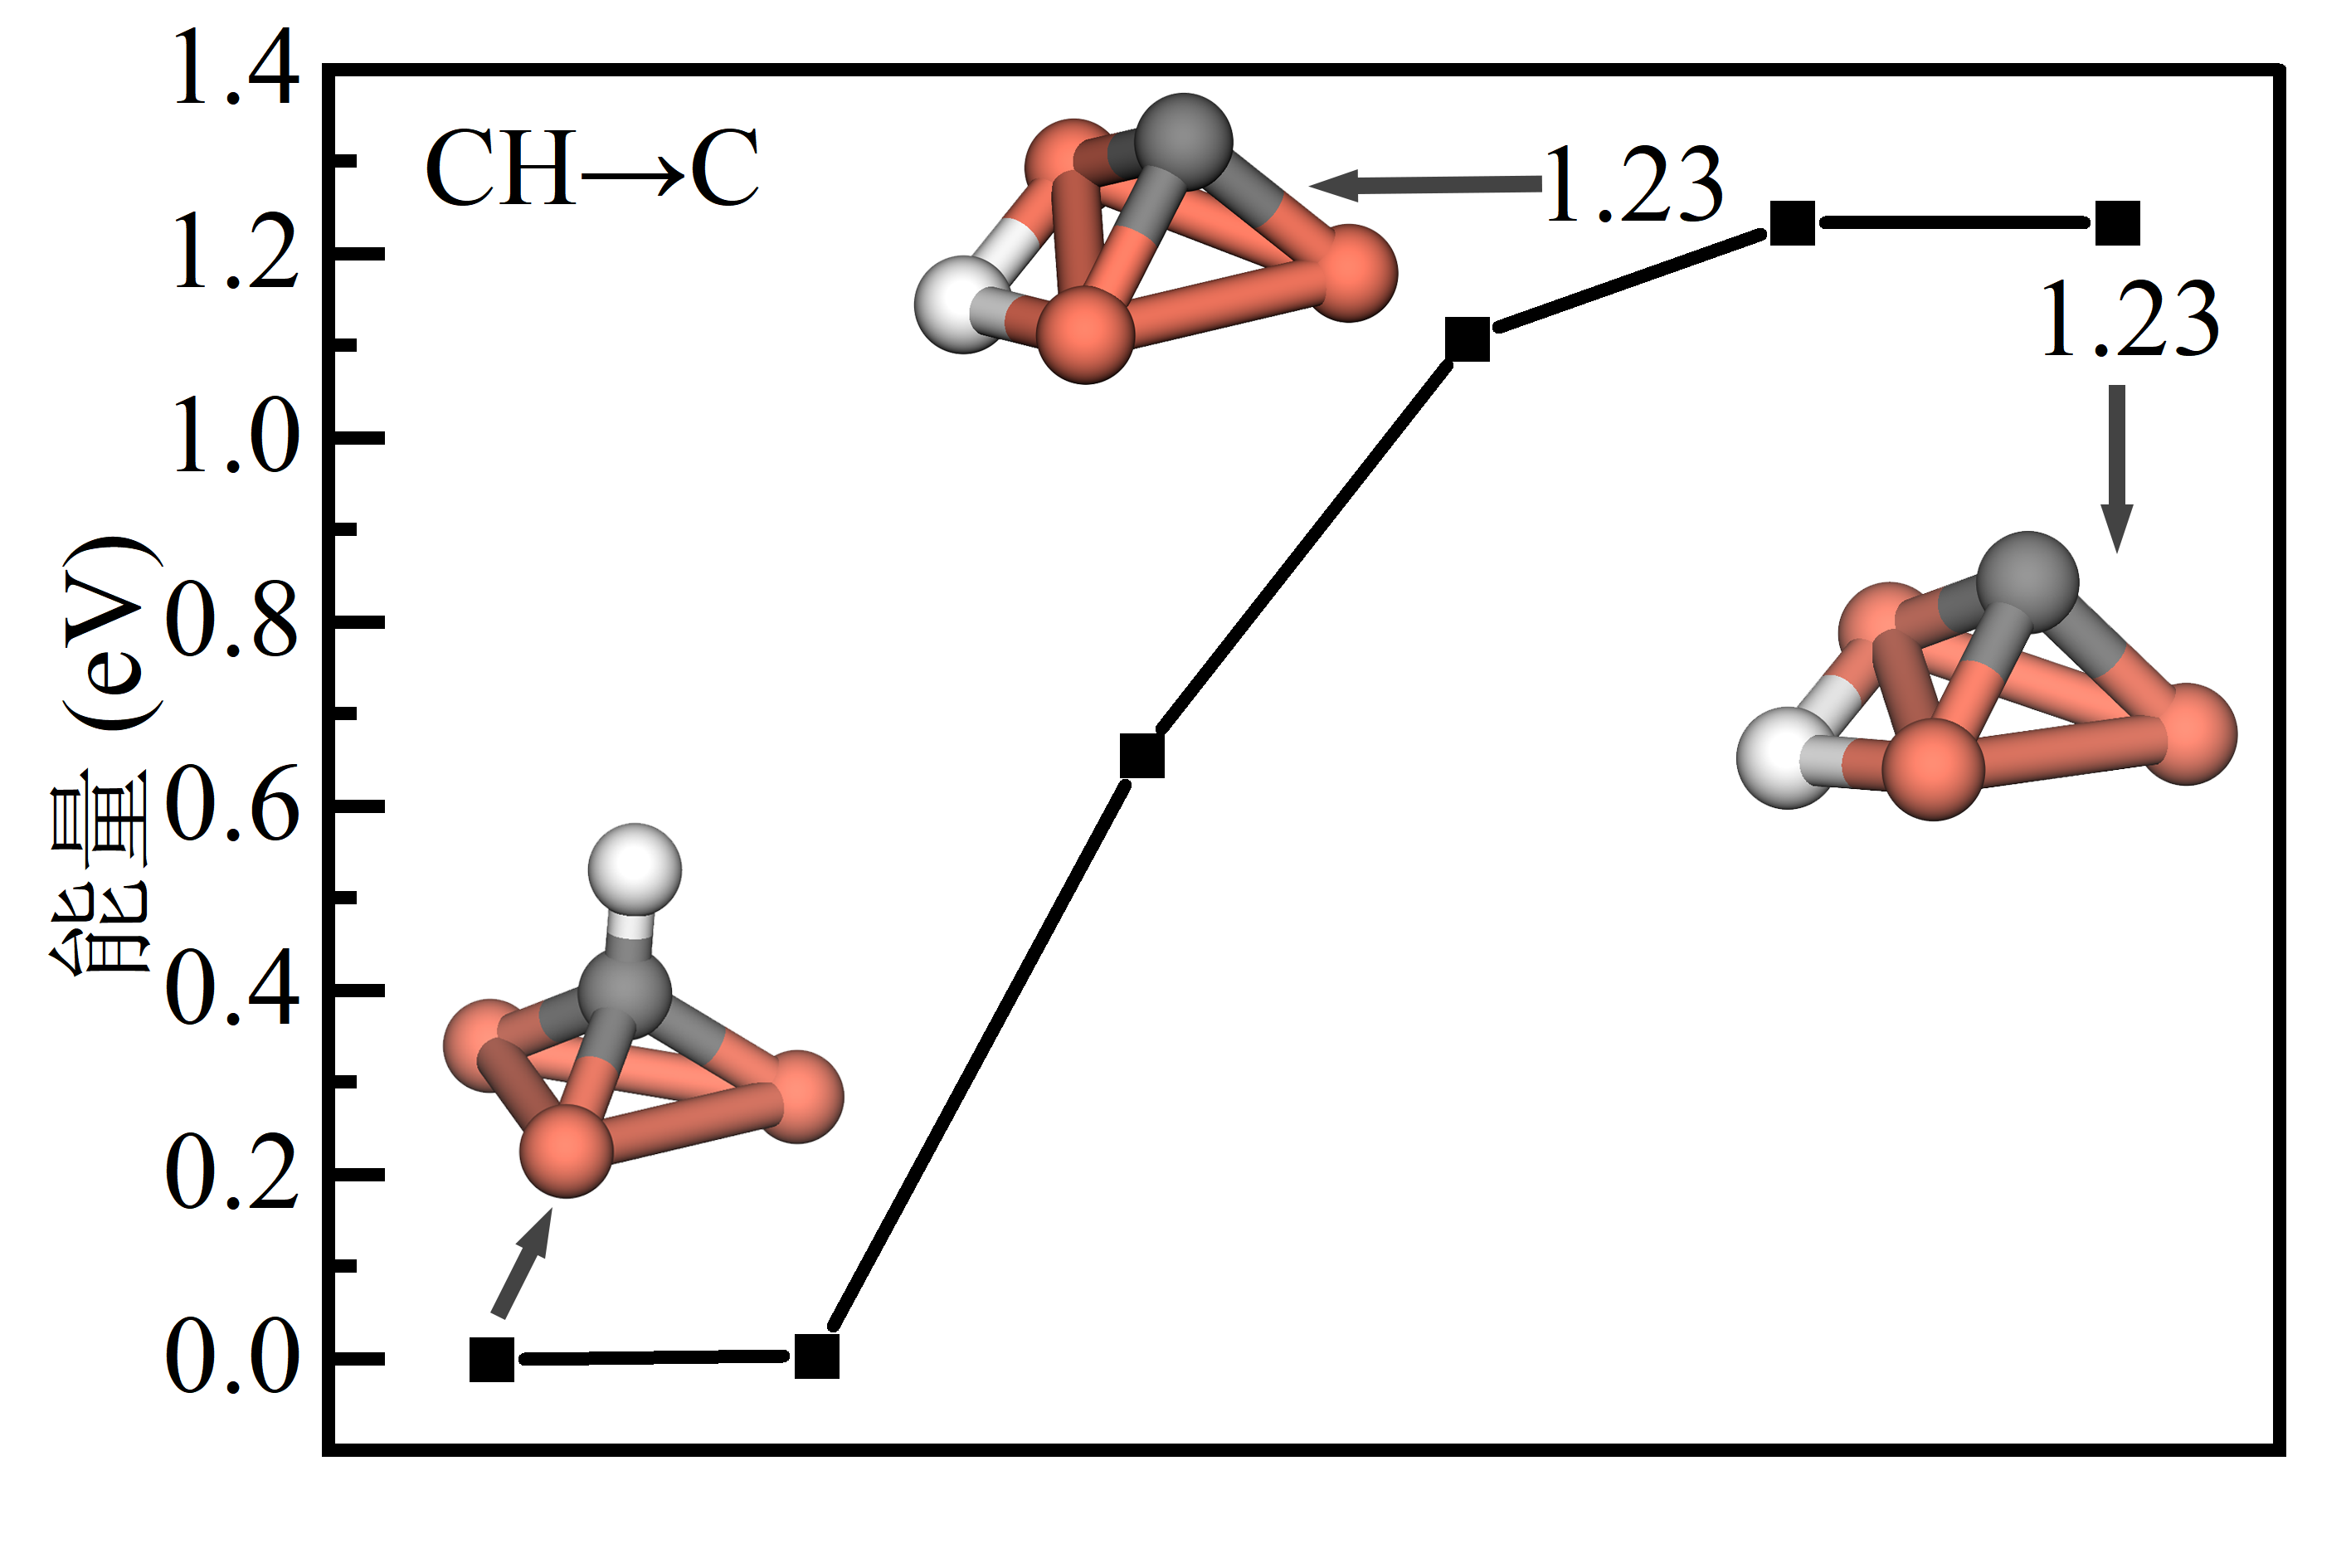
\includegraphics[width=0.45\textwidth]{pic/CG_DFT_Cu3-CH-C.png}
        }
        \caption{\cemb{Cu3}团簇表面\cemb{CH4}脱氢解离的四个反应步骤的反应过程以及能量变化。(a)\cemb{CH4 -> CH3 + H}反应;(b)\cemb{CH3 -> CH2 + H}反应;(c)\cemb{CH2 -> CH + H}反应;(d)\cemb{CH -> C + H}反应。在原子结构中,铜原子为橙色;碳原子为灰色;氢原子为白色。}
        \label{fig:CG_DFT_Cu3-CH4-C}
    \end{figure}

    在图\ref{fig:CG_DFT_Cu3-CH4-C}中,我们绘制了在\cemb{Cu3}团簇表面\cemb{CH4}脱氢解离的四个反应步骤的反应过程以及能量变化图。可以看到,在\cemb{Cu3}团簇的表面,\cemb{CH4}吸附在\cemb{Cu}三角形的顶点处,\cemb{CH4}脱氢的过程也在这个顶点\cemb{Cu}原子上发生。在\cemb{CH4}脱氢为\cemb{CH3}的过程中,\cemb{CH4}中的一个\cemb{H}原子朝\cemb{Cu}三角形的一个棱边运动,剩下的\cemb{CH3}部分也在\cemb{Cu}顶点原子的作用下朝三角形的另一个边运动。这个过程需要吸收\SI{0.92}{\electronvolt}的能量跨越势垒。当脱氢的过程完成后,\cemb{CH3}和脱离的\cemb{H}原子分别立于\cemb{Cu3}团簇三角形的两边。\cemb{C}和脱离的\cemb{H}原子分别和两个\cemb{Cu}原子成键,这步反应需要吸收\SI{0.05}{\electronvolt}的能量。对于\cemb{CH4}在\cemb{Cu3}团簇上脱氢裂解的决速步,\cemb{CH3 -> CH2 + H}反应,在初始状态下\cemb{CH3}在\cemb{Cu3}的\cemb{Cu}三角形顶角吸附。在脱氢的过程中,\cemb{CH2}原子团首先移动到\cemb{Cu3}三角形的棱边处和两个顶角的\cemb{Cu}原子成键,此时脱离的\cemb{H}原子在原顶角的位置与\cemb{Cu}相连。移动到这个过渡态至少需要吸收\SI{1.54}{\electronvolt}的能量。随后分离的\cemb{H}原子继续向\cemb{Cu3}三角形的棱边移动,释放出部分吸收的热量,最终在另一个棱边处完成此步脱氢反应,最终消耗\SI{0.76}{\electronvolt}的能量。
    
    在\cemb{CH2}的脱氢反应中,\cemb{CH2}原子团稳定在\cemb{Cu3}三角形的棱边处。反应开始后,\cemb{CH}原子团和分离的\cemb{H}原子分别从\cemb{Cu3}三角形面外绕行的方式进行运动。在攀上了势垒为\SI{1.53}{\electronvolt}的过渡态后,\cemb{CH}原子团位于\cemb{Cu3}三角形表面的中心位置,\cemb{C}原子同时与三个\cemb{Cu}原子具有相互作用,而\cemb{H}原子保持在与一个顶角\cemb{Cu}相连的位置,但也朝向\cemb{Cu3}三角形面的法线方向。随后,\cemb{H}原子继续向\cemb{Cu3}三角形的棱边运动,最终在棱边处于两个顶角的\cemb{Cu}原子成键。此步反应的反应吸热为\SI{1.05}{\electronvolt}。在最终的脱氢步中,过渡态和反应终态极为接近,\cemb{CH}原子团吸收了\SI{1.23}{\electronvolt}的能量后与最后一个\cemb{H}原子分离,形成具有高活性的\cemb{C}吸附原子。
    
    \subsection{\cemb{h-BN}表面石墨烯的生长演化机理}
    
    \begin{figure}[htb]
        \includegraphics{pic/CG_DFT_C_cluster_onBN.png}
        \caption{}
        \label{}
    \end{figure}

    \begin{figure}[htb]
        \subfloat[]{
            \includegraphics{pic/CG_structure_3C.png}
        }
        \subfloat[]{
            \includegraphics{pic/CG_structure_4C.png}
        }\\[-0.5ex]
        \subfloat[]{
            \includegraphics{pic/CG_structure_4CL.png}
        }
        \subfloat[]{
            \includegraphics{pic/CG_structure_5C.png}
        }
        \caption{}
        \label{}
    \end{figure}

    \begin{figure}[htb]
        \subfloat[]{
            \includegraphics{pic/CG_structure_6CH.png}
        }
        \subfloat[]{
            \includegraphics{pic/CG_structure_6CL.png}
        }\\[-0.5ex]
        \subfloat[]{
            \includegraphics{pic/CG_structure_10CR.png}
        }
        \subfloat[]{
            \includegraphics{pic/CG_structure_12C2L.png}
        }
        \caption{}
        \label{}
    \end{figure}

    \begin{figure}[htb]
        \subfloat[]{
            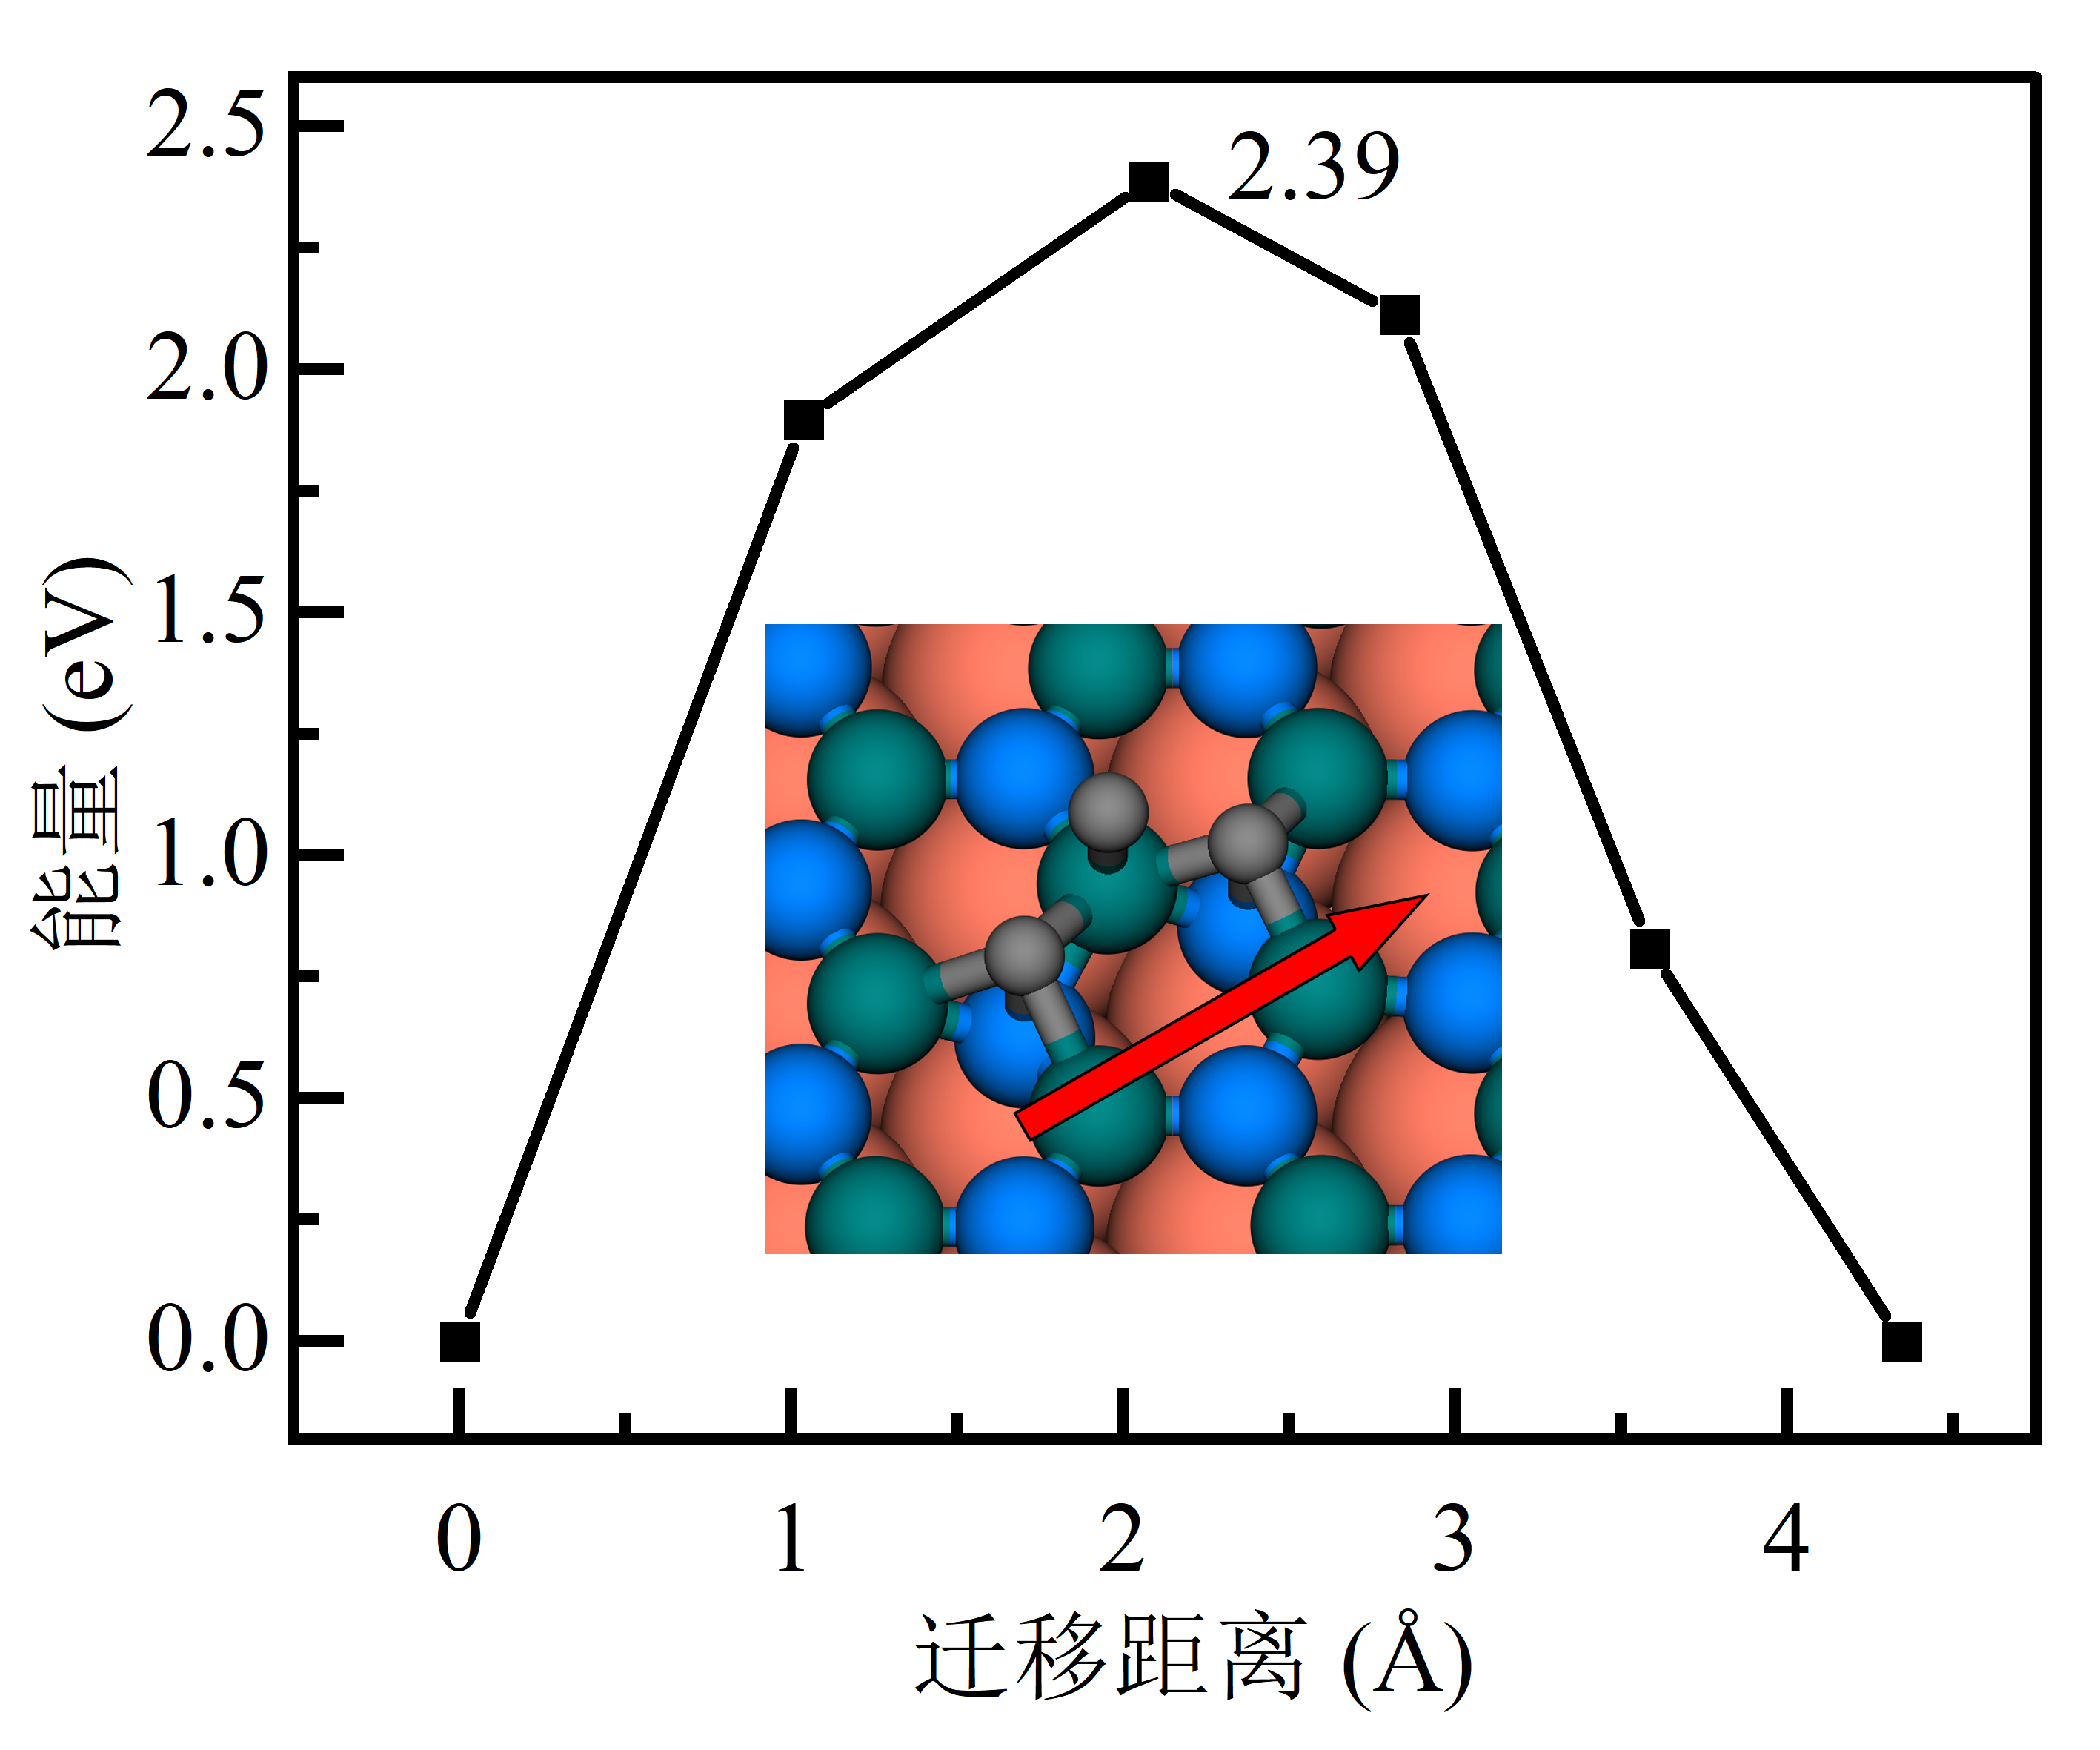
\includegraphics{pic/CG_DFT_CdiffonHBNCu.png}
        }
        \subfloat[]{
            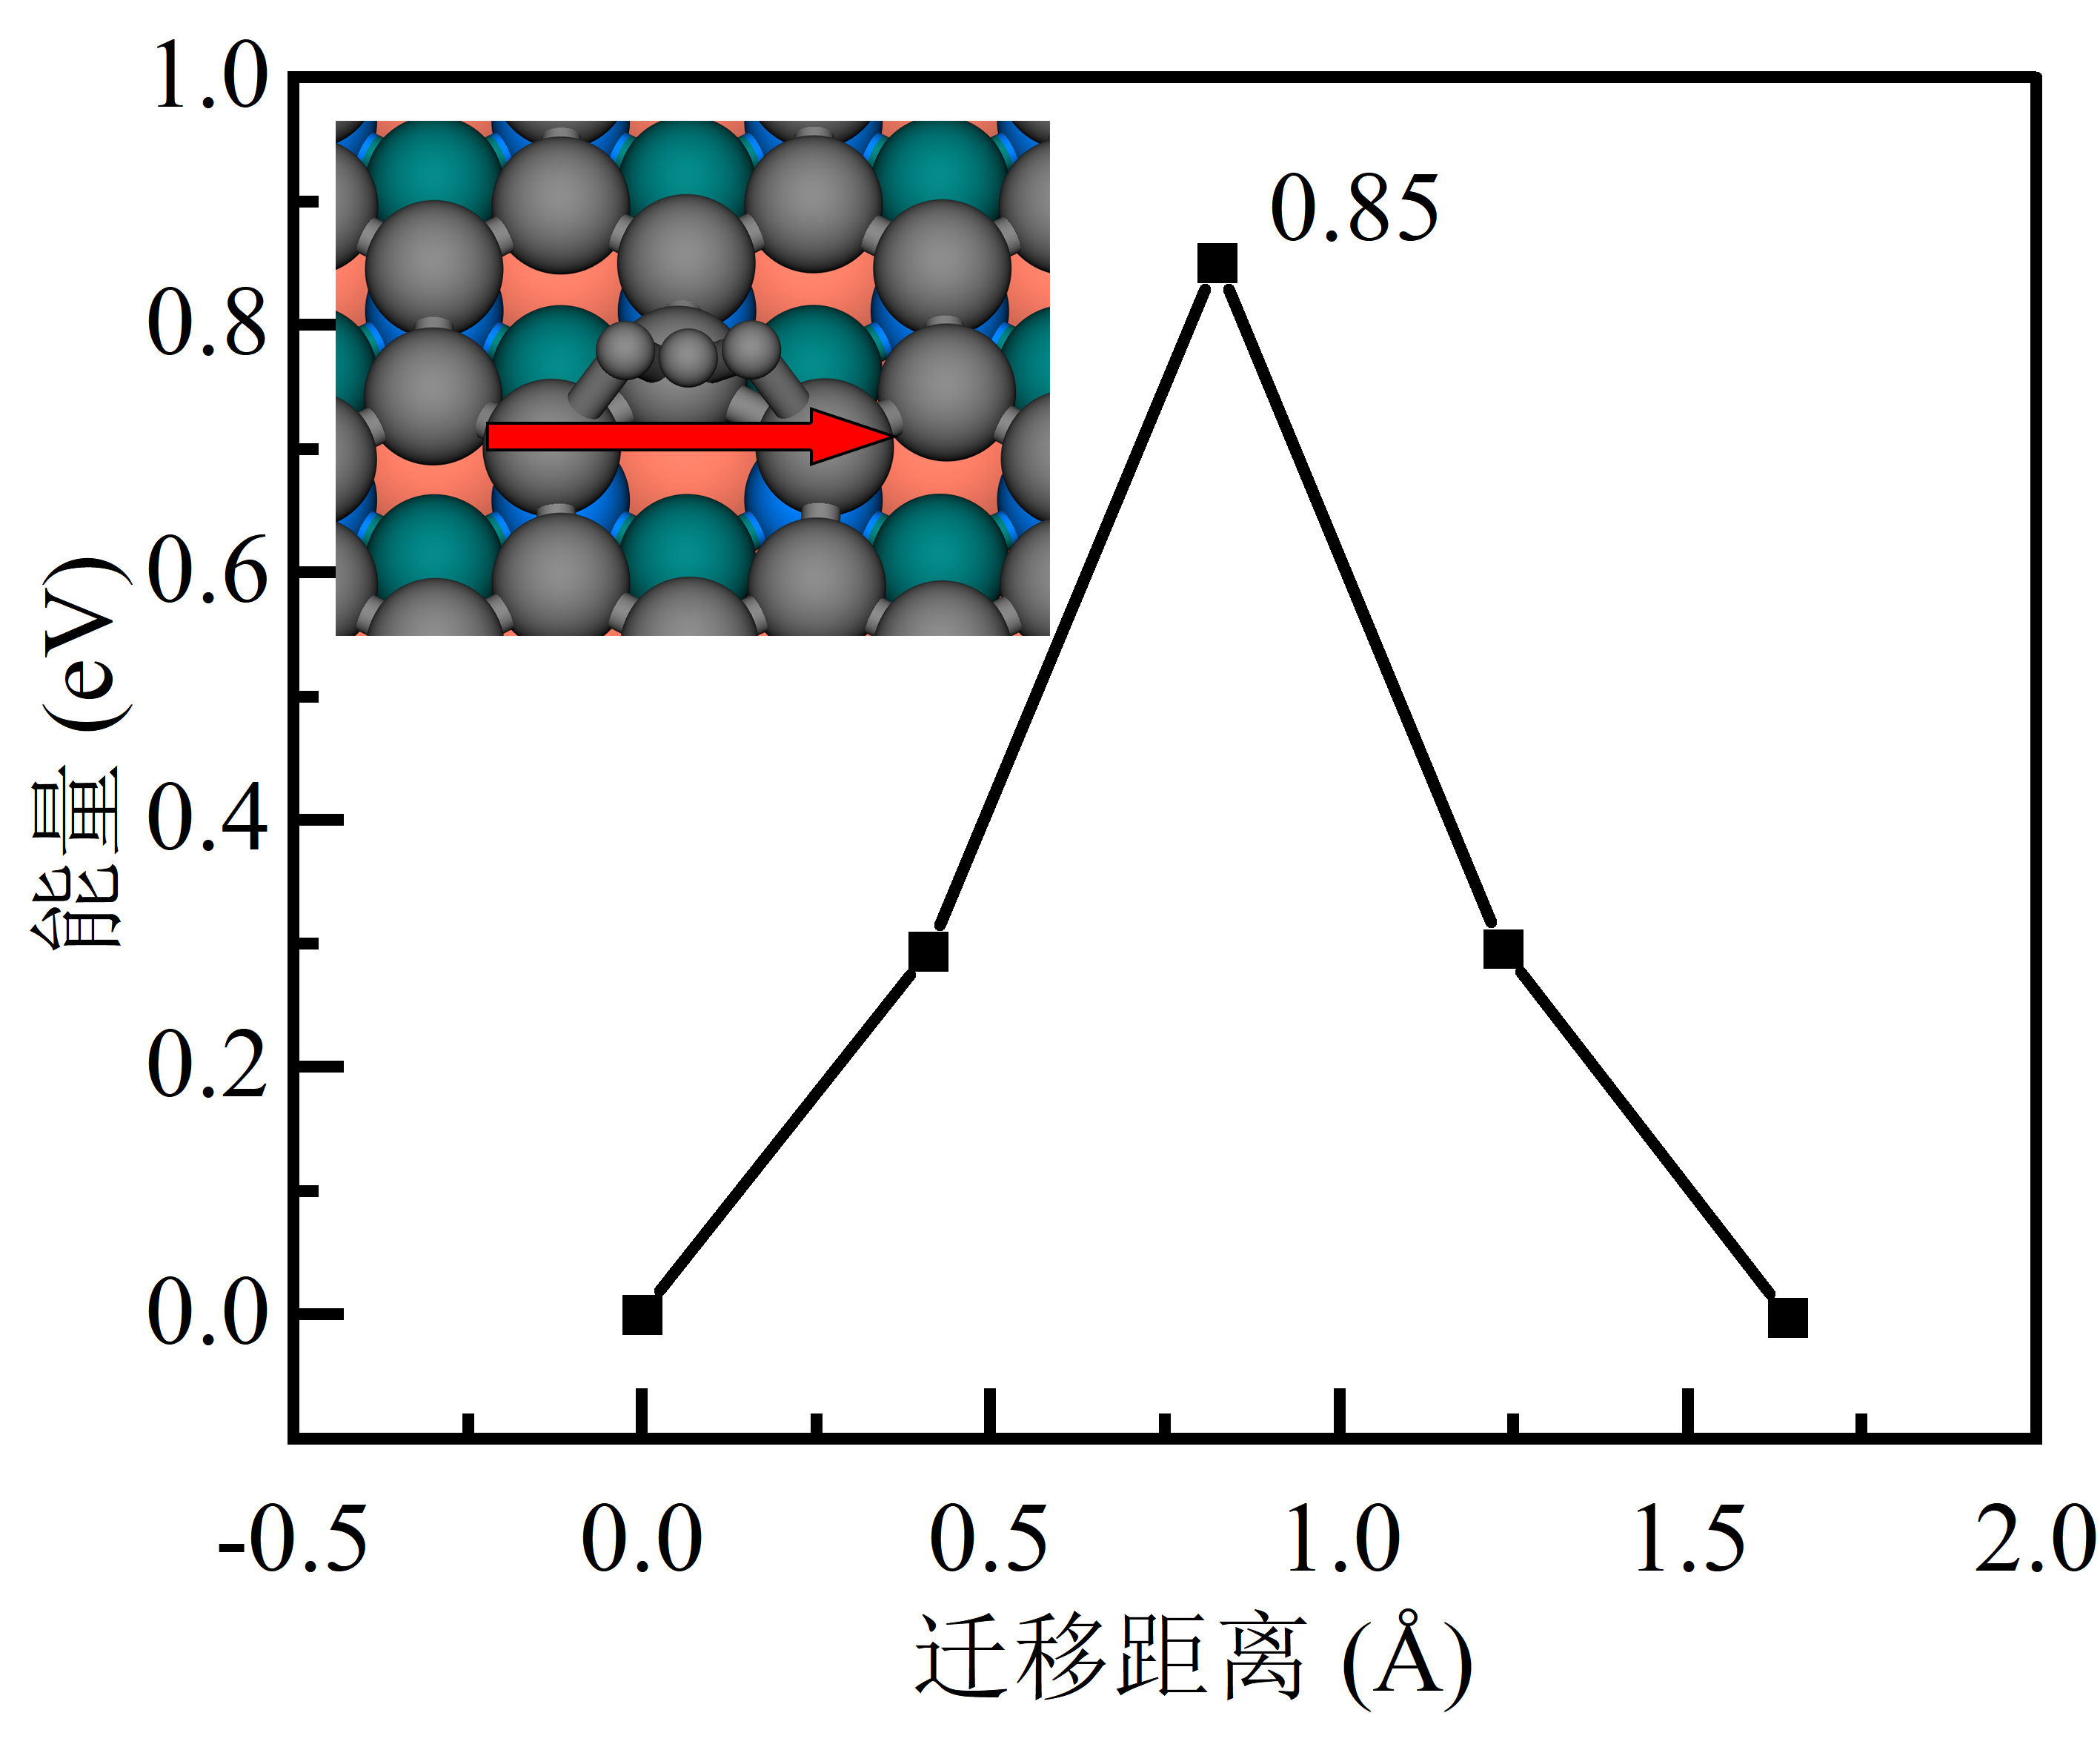
\includegraphics{pic/CG_DFT_CdiffonGhBNCu.png}
        }
        \caption{}
        \label{}
    \end{figure}
    
    \begin{figure}[htb]
        \subfloat[]{
            \includegraphics{pic/CG_structure_13CH.png}
        }
        \subfloat[]{
            \includegraphics{pic/CG_structure_14CR.png}
        }\\[-0.5ex]
        \subfloat[]{
            \includegraphics{pic/CG_structure_16CR.png}
        }
        \subfloat[]{
            \includegraphics{pic/CG_structure_18C2L.png}
        }
        \caption{}
        \label{}
    \end{figure}

    \begin{figure}[htb]
        \subfloat[]{
            \includegraphics{pic/CG_structure_19CR.png}
        }
        \subfloat[]{
            \includegraphics{pic/CG_structure_19CH.png}
        }\\[-0.5ex]
        \subfloat[]{
            \includegraphics{pic/CG_structure_22CH.png}
        }
        \subfloat[]{
            \includegraphics{pic/CG_structure_24CH.png}
        }
        \caption{}
        \label{}
    \end{figure}
\section{石墨烯/二硒化钒横向异质结的生长机理}
\section{总结}